% This file should be replaced with your file with an thesis content.
%=========================================================================
% Authors: Michal Bidlo, Bohuslav Křena, Jaroslav Dytrych, Petr Veigend and Adam Herout 2019


%TODO MAYBE IT WOULD BE NICE TO MENTION ERRORS OF BIOMETRIC AUTHENTICATION - FMR, FAR, FNMR, DET, FRR

\chapter{Introduction}

Blockchain and biometrics are two of the most exciting technologies of the recent era. Blockchain technology is still considered to be in its early stages, but some scientists and experts are already comparing it with the revelation of the Internet in the late 20th century \cite{DecentralizedNetworksFutureInternet}. Just as the Internet revolutionized the way we share information, blockchain technologies have the potential to transform/evolve the way we exchange, store and authenticate information \cite{DecentralizedNetworksFutureInternet}.

The origin of blockchain technology is rooted in the invention of Bitcoin in 2008 by Satoshi Nakamoto \cite{nakamoto2012bitcoin}, where Bitcoin is described as a payment network system designed to make payments accessible and transparent to everyone with the guarantee that their transfers cannot be reversed in any way. With the Bitcoin revelation, a race for the other possible use cases began. It is currently one of the leading innovations in the finance industry \cite{blockchainInFinance}, where the blockchain is the backbone of a new type of monetary system known as cryptocurrencies. Through the use of advanced cryptography, cryptocurrencies similar to Bitcoin promise to reduce fraud, ensure fast, secure, and transparent transactions, lower overall costs, and eventually help manage risk within the joint global financial system. With market capitalization reaching as far as trillions of dollars\footnote{\url{https://coinmarketcap.com/charts/}}, its experiencing a rapid upward popularity trend. The financial sphere use case is not blockchain's only limitation. In addition to monetary transactions, nothing prevents other digital data from being stored on the blockchain \cite{BlockchainAndBiometrics}. This aspect opens up the potential to enable a transformation of entire operational models in well-established fields such as transportation \cite{blockchainInTransportation}, retail\cite{blockchainInRetail}, healthcare\cite{blockchainInHealthcare} or real estate management \cite{blockchainInRealEstate}. 
% TODO I think there is too much unimportant information, maybe reduce it, the intro should be on one page
Biometric systems might also be a field that can benefit from their integration with blockchain technology. Biometric systems are technological systems that allow recognition of an individual by given characteristics such as a fingerprint, voice, or iris.  Existing research on the security of biometrics with the use of blockchain technology focuses mainly on the security of templates \cite{SecuringBiometricAuthenticationBlockchain, BlockchainAndBiometrics, BiometricsOnBlockchain}. 

This thesis investigates the possibilities of securing the biometric system's components of Matcher and Feature Extractor by distributing their execution among a peer-to-peer network that settles on the given operation outcome that is afterward stored in a blockchain. In this way, the execution of the system's processes is decentralized among more participants, resulting in the elimination of a single point of failure vulnerability, common for traditional biometric systems. The use of blockchain builds trust in the network and allows auditability and traceability of executed procedures in previous components, with the intention of minimizing possible attacks on transmission channels (e.g., ``replay attacks'') or to reveal incidents of attempted security breaches. The communication and fundamental functionalities of the proposed system were demonstrated and implemented as a console program.


\chapter{Theory}
\section{Biometric systems}
\label{Biometric systems}
Day in and day out, we use our senses to recognize others by our visual characteristics, such as facial looks, voice, or even the style and cadence of walking. Due to this fundamental ability, we can build relationships and trust, which is an essential function of our being. This natural fact was one of the reasons why scientists in the 1960s started to research automated personal identification \cite{biometricsHistory}.

Biometrics or biometric technologies represent procedures that observe, recognize, and measure selected attributes and characteristics of a living individual or a group of individuals to identify their unique properties. These characteristics are not stored in their pure form, but in the form of preselected features also called templates (i.e., selected features, mathematical model, or the biometric sample by itself). They represent a persistent bond between a person and his identity. The standardized definition according to ISO/IEC 2382-37 \cite{isoBiometricSystem} is ``the automated recognition of individuals based on their biological and behavioral characteristics''.
Biometric systems can greatly increase security and convenience, compared to traditional recognition systems based on passwords, pins, or smart cards \cite{BiometricRecognitionSecurity}. They might prevent impostors from accessing restricted areas or resources or reveal criminals trying to hide their real identities. With advances in their research, real-world use cases of biometric systems are becoming more frequent. They are used in many sectors, such as airport security, mobile access and authentication, building access control, law enforcement, or banking.

\label{BiometricTypicalProcesses}
Biometric systems usually have two phases of operation: enrollment and recognition\cite{BiometricAuthentication}. To register new users, the enrollment phase ensures that the system stores and logically links individuals to their biometric data (template, mathematical model, or biometric sample by itself) in a database. In recognition, previously stored reference information is compared with the user's newly acquired biometric data, and the authentication result is determined.

Although the leakage of the original biometric information is minimized by using templates, it can still be estimated by reverse engineering\cite{BiometricTemplateSecurity}. This fact is especially important to keep in mind when researching options for biometric integration with immutable data structures such as the blockchain \cite{BiometricsOnBlockchain}.

%in need of pages, you can mention applications of biometric systems%

\subsection{History}
The term ``Biometrics'' consists of two separate words, each with roots in Greece. The first part ``Bio'' originated from \emph{bios}, as in ``living constituents'' or ``biological'', which refers to living organisms and their physiological or behavioral traits. Although the word ``metrics'' comes from \emph{métrique}, it refers to measurements or quantitative analysis. Historically, the term ``biometrics'' has been known to be a field of biology focused on the measurable analysis of statistical biological data. Today, a more frequent interpretation of ``biometrics'' is ``biometrics authentication''\cite{wayman2005biometric}, mainly due to its use in the security field. 

The first developments of systems with automatic human recognition (authentication) date back to the early 1960s. The very first biometric research appeared in the journal \emph{Nature} published by Mitchell Trauring in 1963. Instead of referring to ``biometrics'', the article mentions only ``automatic fingerprint recognition''. The article states that automatic fingerprint recognition could provide personal verification with faster operating times or lower costs, since no skilled operating personnel is needed.
In the 1970s, the field was already known as ``automatic personal identification''. The United States (U.S.) National Bureau of Standards (NBS) put a great emphasis on its research, and in 1970 started formal testing of fingerprint systems. Later on, other U.S. organizations including the U.S. National Academy of Sciences (NAS, today NIST) or the U.S. Air Force followed suit.
The first reference to the term ``biometrics'' was found in the 1981 newspaper article in The New York Times \cite{RecognizingTheRealYouTNYT1981}, where the potential utilization of physiological traits to verify a person's identity was discussed. It is intended to improve existing security systems by replacing the standard authentication methods, which depend on something you possess (plastic cards, keys, etc.) or something you remember (passwords, pins, etc.), with biometrics that do not require such methods. Instead, it introduces a much more convenient method, which depends on who you are or what you do. This brought many advantages as you don't have to remember the passwords or you are not being forced to carry a special object with you to get verified. But it also has its downsides (e.g., data breaches, privacy issues).
In the 1990s, the greatest progress was made by developing improvements in iris recognition \cite{biometricsHistory}. During those years, the biometric community began to grow, new organizations were created, and conferences were held presenting new research. In 1991 the first European organization called the Association for Biometrics (AFB) was founded.
In the 21st century, biometrics has attracted great interest in passenger applications. Countries such as the United States, the United Kingdom, and Germany piloted their projects for air travelers, and several countries plan to issue passports with chips that hold biometric data.

\subsection{Authentication}
\label{Authentication}
Biometric systems are a single special instance of systems that perform user authentication. Other authentication systems (access control systems) use methods such as passwords, one-time passwords, or radio frequency identification (RFID). All of these systems operate with similar fundamentals of authentication. Bishop in his book\cite{ComputerSecurityBishop} defined authentication as \emph{``authentication is the binding of an identity to a subject.''}.
The authentication process is then a security process that identifies subjects who request access to the secure system, network, or device. The management of access control determines the subject's identity using information that the subject knows (username and password), something that the subject owns (USB, mobile phone, or smart card), or something that qualifies the subject (biometrics such as face, fingerprint), or something that the subject can do (signature, walk)\cite{BiometricAuthentication}. All of this information must be stored and managed in the system.
Authentication systems can be modeled as a signal-based model consisting of three components\cite{SecuritForBiometricData}: the human subject, the authentication system, and the reference storage. Components communicate through certain transmission channels, each with its purpose. The visualized model can be seen in Figure \ref{signalModel}.

\begin{figure}[ht]
	\centering
	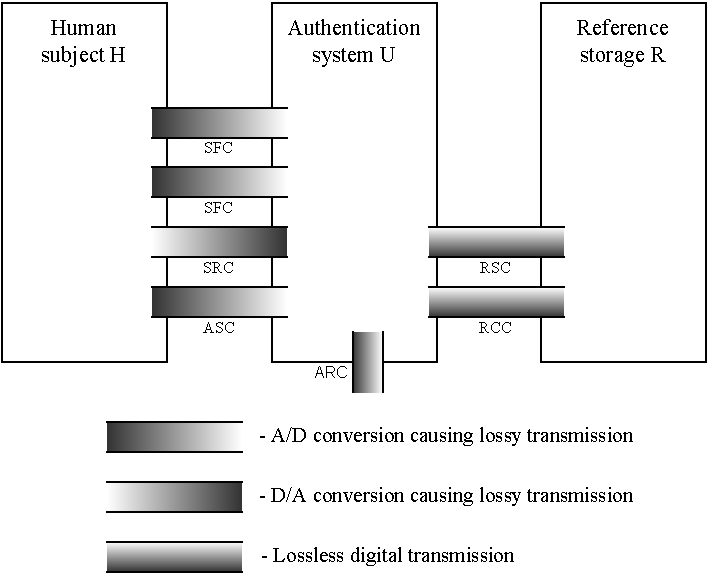
\includegraphics[width=0.8\linewidth]{obrazky-figures/SignalAuthenticationModel.pdf}
	\caption{Generic signal model for authentication systems.}
	\label{signalModel}
\end{figure}

The human subject or user is the individual trying to access the system by authenticating its identity. To do so, the individual provides the requested authentication information to the authentication system. The authentication system then processes the provided data and, depending on the execution process, the components communicate, exchange information, and transmit data with each other. The model presents all data flow channels between those components needed for classical authentication systems or response-based systems (the user authenticates on a challenge from the system, e.g. biometric authentication). Because the subject's entered data are transferred to the system from the real world, the transmitted information is subject to analog-to-digital or digital-to-analog conversion, and thus loss of information may occur. Communication channels between authentication systems and reference storage are considered to be lossless due to transmitted information being digital. Each of these channels and components may be vulnerable to attacks, and therefore their protection is required (as discussed in Section \ref{Biometric system's security}), and the role of the channels is described below.

\begin{itemize}
  \item{Authentication submission channel (ASC) - Transmission of the authentication information from human subject to authentication system(use of this channel is mandatory in all authentication cases, for authentication by identification its even sufficient).}
  \item{Synchronization forward channel (SFC) - Transmission of accompanying additional information from authentication system to human subject (required for verification or challenge-response authentication systems).}
  \item{Synchronization reverse channel (SRC) - Authentication system requests human subject to provide certain information.}
  \item{Reference information control channel (RCC) - Authentication system requests storage for reference information(eg. username and password).}
  \item{Request information submission channel (RSC) - The reference storage transmits requested information to authentication system.}
  \item{Authentication result channel (ARC)- Delivers the authentication result (eg. user access denied).}
\end{itemize}

\subsection{Structure of biometric system}
A Biometric system can be considered as a pattern matching system that operates by collecting biometric raw data from an individual, extracting distinguishable feature sets from this data, comparing the extracted feature sets with previously stored feature sets, and providing the result of the comparison with the external application. Conventional biometric systems are described as a model consisting of five modules, each performing one essential operation: a sensor module, feature extractor module, matching module, and a template or feature set database \cite{HandbookOfBiometrics}. Sometimes, the application module is left out of the models representing the biometric system, but for the sake of showcasing all possible weak points later on, we kept it here. The modules and their communication hierarchy are modeled in a Figure \ref{biometricSystem} and their roles are described in the list below \cite{AttacksOnBiometrics, HandbookOfBiometrics, BiometricSystemsBook}.

\begin{figure*}[h]
	\centering
	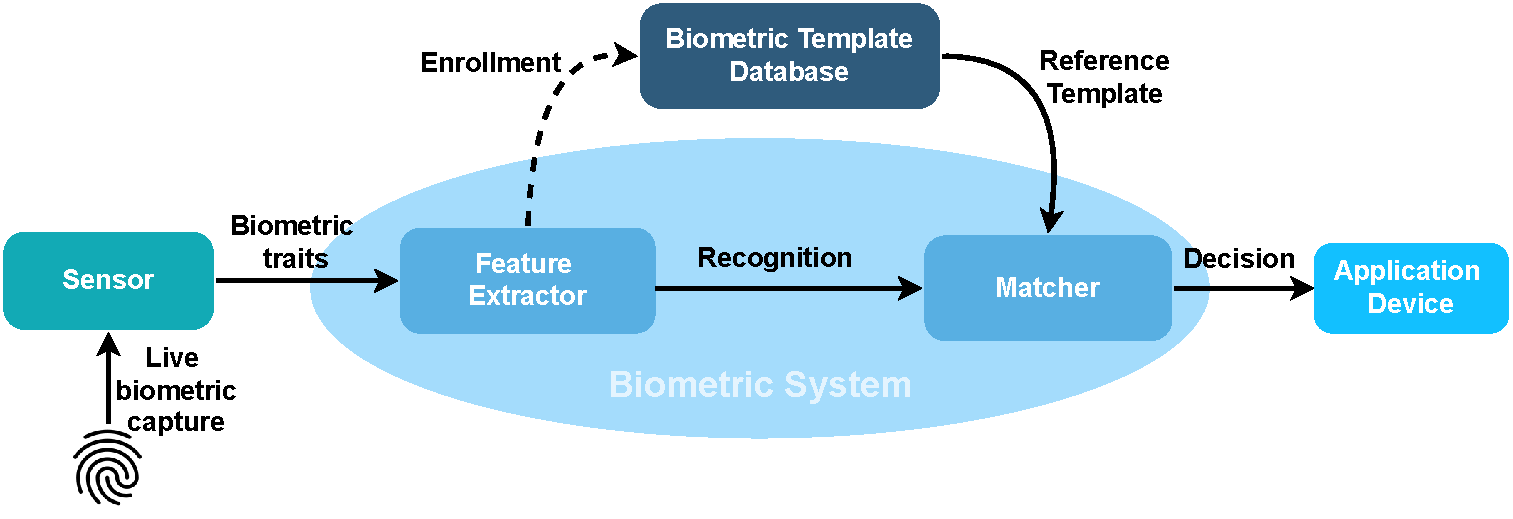
\includegraphics[width=\linewidth]{obrazky-figures/BiometricSystem.pdf}
	\caption{Schema of biometric system and it's processes.}
	\label{biometricSystem}
\end{figure*}

\label{BiometricModules}
\begin{enumerate}
    \item \textbf{Sensor module} - Processes the raw biometric data of an individual and converts them into digital form (e.g., the image of a fingerprint or face). After conversion, the acquired data are transmitted to the feature extraction module.
    The sensor module is the point of human-computer interaction. Therefore, it must define a suitable user interface according to the acceptability criteria to reduce the failure rate with biometrics collection. 
    \item \textbf{Feature extraction module} - Within feature extraction, several filters and quality enhancement algorithms preprocess the raw data to simplify extraction. If the received features are of poor quality, the feature extractor might ask the individual to use the sensor again. Otherwise, the data is processed to search for compact distinctive characteristic points known as features. These features can be incorporated into templates (that is, features on their own, parameters of a mathematical model characterizing the features \cite{BiometricAuthentication}). During the identification or verification process, the templates are transmitted to the matching module to complete the recognition. In the case of enrollment, the extracted features are transmitted and stored in the database module.
    \item  \textbf{Matching module} - The received template is compared with previously stored reference templates, scores are generated and used for the verification/identification decision. The variance of biometric data requires the execution of ``fuzzy comparisons'' by using predefined thresholds determined by score distributions between authentic and artificial subjects.  Depending on the execution mode, the matcher either: (1) compares the received features with all the templates stored in the database (identification) to search for an enrollee with the highest score. If the score is below a predefined threshold, the identification failed.
    (2) compares the received features with the template of the claimant (verification). The predefined threshold is used again to determine the genuineness of the claimed identity. In some articles, this module is separated into matching and decision modules, where the matching module generates scores, and the decision module applies the threshold to determine the authentication outcome. %TODO in some articles maybe requires to cite some
    \item  \textbf{Template database} - Also known as data storage, is responsible for saving references to biometric information (i.e., templates, samples, or models) paired with some biographic information (e.g.,ID, PIN, or name) about enrollees. Data storage can be centralized (on a server or a computer).
    \item  \textbf{External application} - Application (e.g., entrance to secure area, e-Commerce, or mobile phone) that is secured by the biometric system. 
\end{enumerate}



%\section{Evaluation of biometric systems}

\subsection{Biometric traits}
\label{Biometric traits}
Biometric systems use a variety of inherent physiological or behavioral characteristics (see Figure \ref{BiometricTraitsImages}) such as fingerprints, palm-print hand geometry, veins in hand, gait (gait is a way or style of walking or moving on foot), iris, retina, voice, face, signature, or even keystrokes \cite{biometricTraitsSpec} to perform real-time biometric authentification and identification of an individual \cite{DrahanskyMartin2011B}.

Biometric systems differ in their capabilities, complexity, and performance according to the type of biometric trait used. Some traits are more efficient, some are more reliable than others, but all have to conform to set properties (see the list below). The choice of biometric trait depends on the requirements and criteria of the given application. The main properties of the biometric traits evaluated are\cite{clarke1994human}:
\begin{itemize}
    \item Uniqueness: Biometric traits must be different enough to be distinguishable between any individual.  
    \item Permanence: The trait should remain the same despite the influence of other factors, such as aging, etc. 
    \item Collectability: The trait should be able to be captured easily by anyone and anywhere. 
    \item Acceptability: The selected trait should be socially acceptable to capture. 
    \item Convenience: The collection of the trait should be convenient and methodical. 
    \item Exclusivity: The standalone trait should be sufficient for the entire process of identification.
    \item Cost: The capture, measurement, and evaluation process should be designed in a cost-effective way.
\end{itemize}


\begin{figure*}[h]
	\centering
	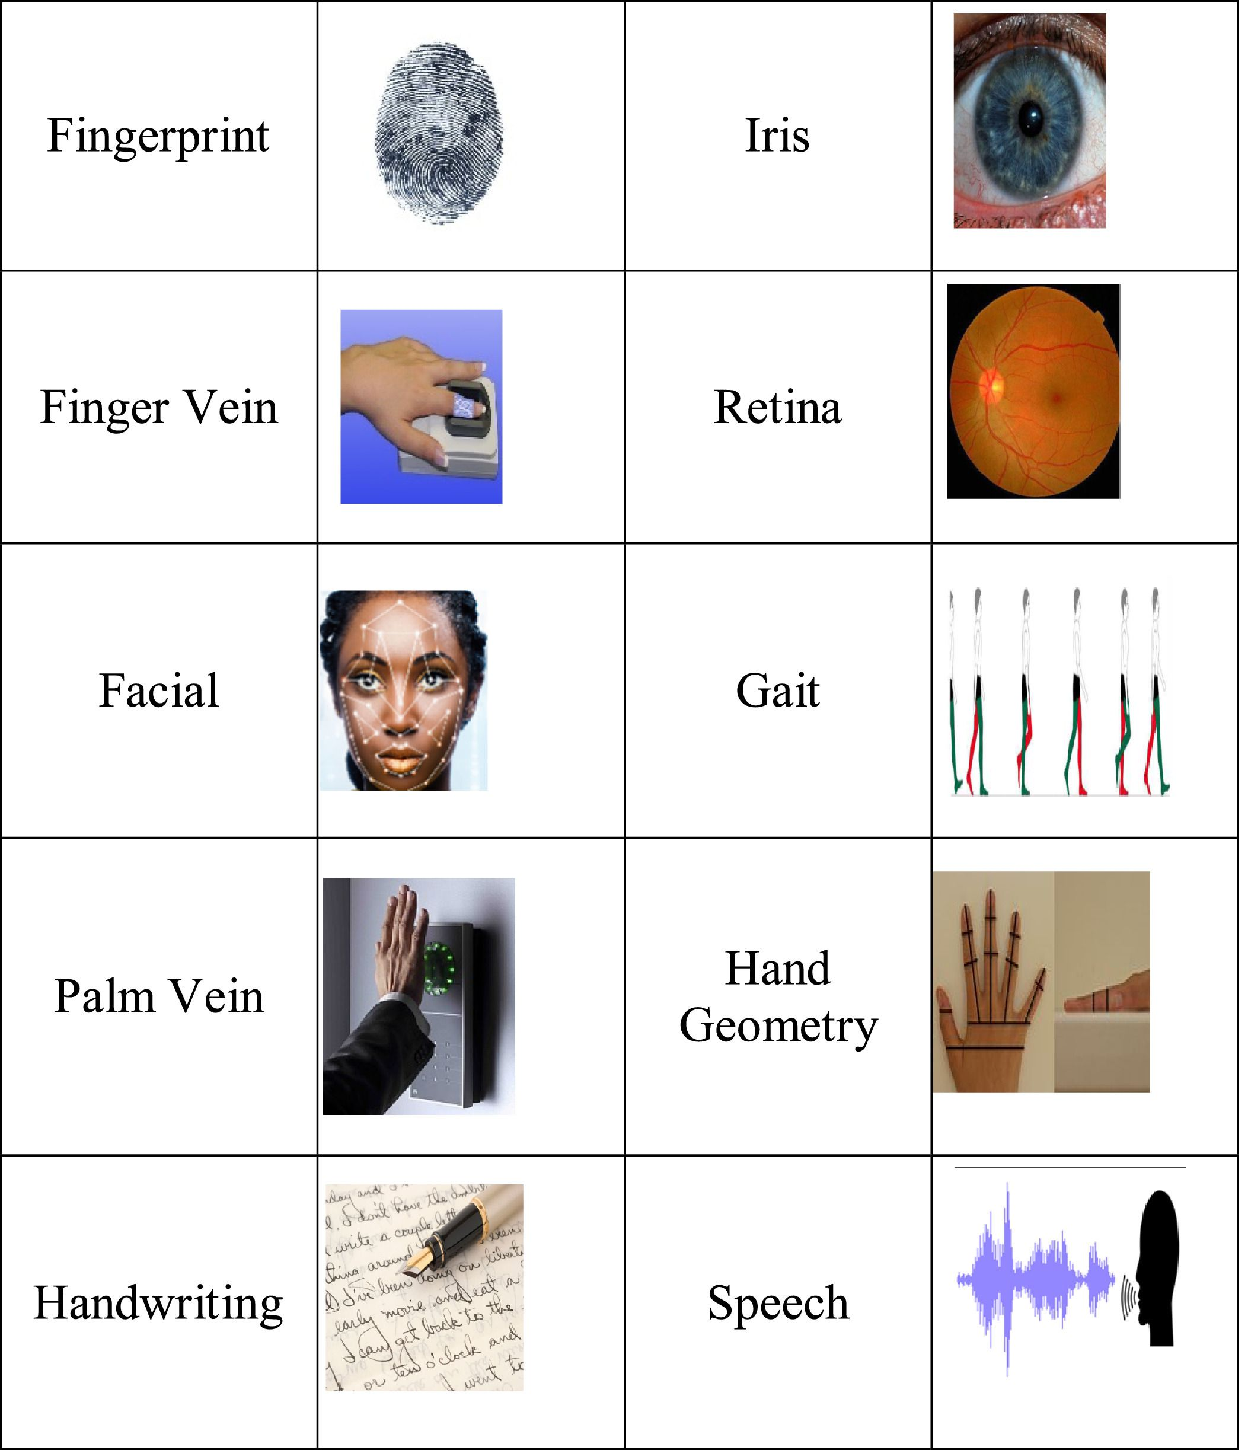
\includegraphics[width=0.56\linewidth]{obrazky-figures/BiometricTraits.pdf}
	\caption{Images showcasing biometric traits. Taken from \cite{biometricTraitsSpec}.}
	\label{BiometricTraitsImages}
\end{figure*}

Biometric systems that use a single biometric trait are called ``Unimodal''. Biometric systems could also utilize more biometric traits, these systems are called ``Multimodal'' or alternatively ``Multibiometric'' \cite{biometricTraitsSpec}. For the acquisition of multiple or complementary traits ``Multimodal'' systems employ a combination of sensors, algorithms, procedures, and modes simultaneously. Compared to ``Unimodal'', the use of ``Multimodal'' systems provides greater security. They are less prone to spoofing attacks and offer better reliability and robustness. Capturing two (or more) different biometric traits could cause discomfort, as each need to be acquired by a different sensor. The usual solution is to pick traits that are in the same body part.  

%TODO possible addition: maybe emphasize here that the storing of biometrics should be handled really carefully(hint that storing in the blockchain, might be risky in the future) %

\subsection{Biometric stages}
Depending on the context of the system, a biometric system generally operates in two stages of operation: enrollment and recognition. The recognition stage requires a prior enrollment of the users to perform their expected execution. Historically, the recognition stage has been classified into two types: identification and verification.  The distinction was made according to the mode of execution of the biometric system: it either authenticates the claimed identity (verification) or it identifies individuals without the claimed identity (identification) \cite{BiometricSystemsBook}. Both the verification and identification stages can be classified by their outcome as a two-class problem: for verification, the subject gets authenticated by having his claim successfully verified or rejected\cite{BiometricSystemBasic}, in identification, the subject's identity gets recognized or classified as unknown to the system. 
Today, use cases (for example, modern ``few-to-many matching'') and ongoing research of biometric systems have reached the point where verification / identification classification is no longer apparent\cite{BiometricSystemsBook}.

\subsubsection{Identification}
Identification mode tries to establish a person's identity without any entered claim. This is achieved by performing a one-to-many comparison of newly captured data with all previously stored data in the system database. In simple terms, the individual asks the system the question ``Who am I?'' or ``Am I already stored in the database?''\cite{BiometricAuthentication}. Identification is essential in negative recognition applications, where the system concludes whether the individual is who he denies being. These applications verify the absence of previous enrollment and aim to prevent the use of multiple identities by the same user. Negative recognition systems are limited to biometrics, as there is no other alternative automatic method to verify a claim of unknown identity\cite{HandbookOfBiometrics}.

\subsubsection{Verification}
Verification mode tests the hypothesis that ``the submitted traits are from an individual already stored in the system'' and validates a person's identity by doing a one-to-one comparison of newly captured data and claimed identity (e.g., with a PIN, magnetic stripe, user name, or smart card) with a previously stored template in the system database. In basic terms, the individual asks the system the question ``Am I the one who I claim to be?''\cite{BiometricAuthentication}. Verification is often used in applications that perform positive recognition, where the aim is to prevent more users from using the same identity. The use of biometrics in positive recognition systems is voluntary, as there are many alternative methods to verify identity claims (e.g., simple passwords, PINs, or keys)\cite{HandbookOfBiometrics}.

\subsubsection{Enrollment}
During this procedure, the trait is acquired by the hardware sensors and then transmitted to the feature extraction module, where feature measurements are taken to create a template that is eventually stored in the database. Within enrollment, biometric information of an individual is linked to his identity (e.g., by ID, PIN, or name). In certain applications, the enrollment process may be supervised by a human. For example, a person who registers a new computer account on his biometric-enabled system can enroll his biometrics without any supervision. In another instance, an application where a person needs to use an ATM with biometric authentication will have to undergo biometric enrollment in the presence of a bank official\cite{HandbookOfBiometrics}. Due to human certification of credentials during enrollment, these applications might additionally store biographic information (such as name, address, phone number, etc.). 

%TODO maybe add here biometric storage options -> see https://www.nec.co.nz/market-leadership/publications-media/how-is-biometric-data-stored/

\subsection{Biometric system's security}
\label{Biometric system's security}
Biometric systems have a great reputation and offer various advantages compared to traditional authentication systems. However, they can still be vulnerable to various attacks. These attacks can be grouped according to their target into four categories: processing and transmission level attacks, input level attacks, back-end attacks, and enrollment attacks\cite{BiometricAuthenticationVulnerabilities}. Transmission-level attacks exploit the fact that the transmission of sensitive data in biometric systems is usually done in networks of local or remote machines. The channels connecting the system thus might be intercepted, and the data may be used for various malicious attacks.
To prevent data alteration, interceptation, or leakage in transit, biometric systems adopted security aspects such as data encryption, anti-spoof measures, and appropriate fallback techniques \cite{BiometricAuthenticationVulnerabilities}. In communication channels where transmission is done through wired cables, improving physical connections in the real world increases transmission security. In input-level attacks, the attacker might replace or interfere with hardware or software and gain access to processing modules of the biometric system (for example, by implementing spyware). The established measures to prevent such attacks include improving the physical protection of devices, integrating mechanisms to prevent software modification, and intrusion detection methods\cite{IntrusionDetection}. Back-end attacks consist of attacks on matching, database, or combination of both modules, targeting modification or replacement of the templates themselves or the authentication decision of the system. Enrollment attacks target the enrollment stage, where the goal is to fool the identity management system of the biometric system by enrolling as someone else with their biometrics or the other way around. The authenticity of the enrollment process should be handled within the organization's procedures. As Figure \ref{BiometricSystemSecurityWeakPoints} shows, there are generally eight weak points that are vulnerable to attacks \cite{AttacksOnBiometrics}. From another point of view, attacks can be classified into two types \cite{AttacksOnBiometrics}:
\begin{enumerate}
    \item \textbf{direct attacks} - referring to attacks that do not require any knowledge of how the authentication system operates internally, they aim at the system interface.
    \item \textbf{indirect attacks} - in contrast to direct attacks, here the knowledge of inner operations is required to be successfully performed.
\end{enumerate}

\subsubsection{Security vulnerable points}
\label{Security vulnerable points}

\begin{figure*}[h]
	\centering
	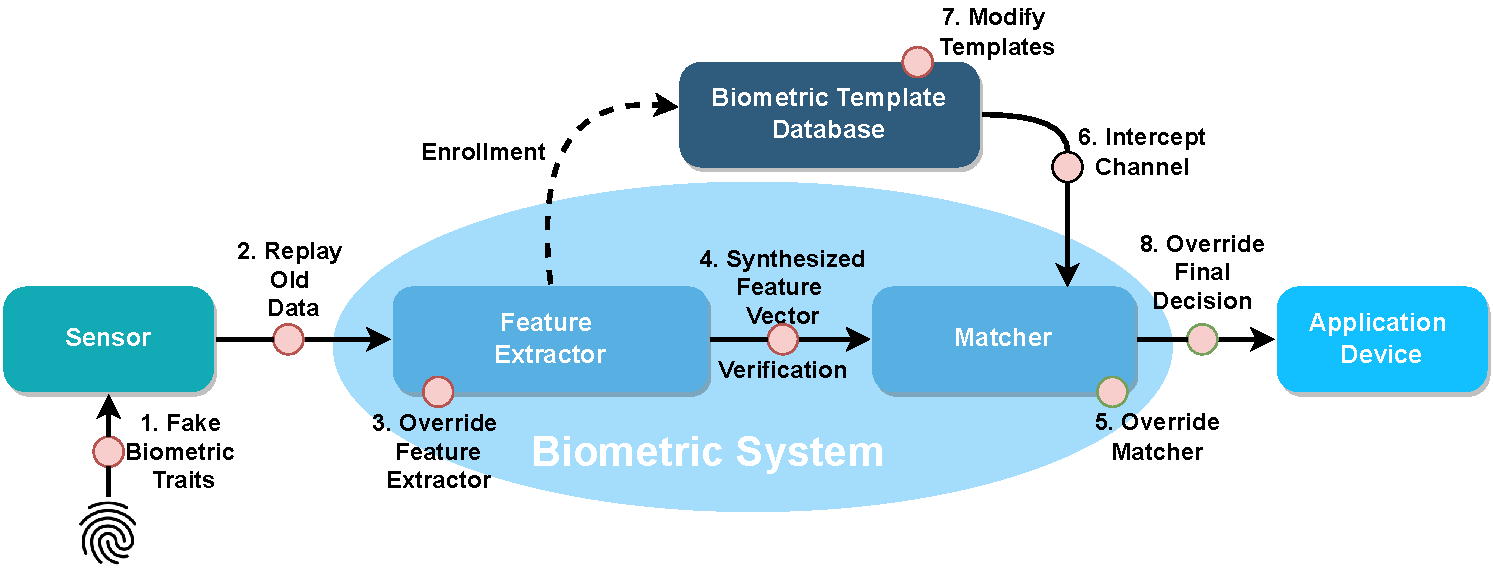
\includegraphics[width=\linewidth]{obrazky-figures/BiometricSystemWeakPoints.pdf}
	\caption{Security weak points in biometric system.}
	\label{BiometricSystemSecurityWeakPoints}
\end{figure*}

\label{Security vulnerable points description}
\begin{enumerate}
    \item \textbf{Type 1 attacks.} Usually targets the sensor module and the authentication submission channel. The sensor could be replaced or integrated with an additional sensor controlled by the attacker to forge biometric authentication. Spoofing is the most common attack. Here, the attacker acts as an imposter and presents artificial biometric data to deceive the biometric system authentication. Other known problematic attacks are ``Overloading'', ``Flooding'' or denial of service (DOS). ``Overloading'' is an attempt to circumvent a system by damaging it or overwhelming the sensor to generate errors. 
     \item \textbf{Type 2 attacks.} Attacks aimed at the channel used to transmit raw biometric data to the feature extraction module. This channel can be intercepted, and transmitted data could be stored for subsequent replay to bypass the sensor. These attacks are known as replay attacks\cite{ReplayAttackDefinition}. In addition to replay attacks, this channel is vulnerable to three other attacks: the eavesdropping attack, the man-in-the-middle attack (MITM), and the brute-force attack.
     \item \textbf{Type 3 attacks.} Also known as attacks on the feature extractor. Here, the attacker might gain control over the feature extractor module, and instead of producing legitimate features, it produces selected features by him. The feature extractor component might as well as the sensor be replaced, resulting in feature processing being done according to the attacker's intentions.
     \item \textbf{Type 4 attacks.} Attack on the communication channel between the feature extractor and the matching module is similar to the second type of attack, vulnerable to replay, MITM, eavesdropping, and brute-force attacks. Again, there is a risk that the attacker can replay intercepted data, in this case, feature values of legitimate users.
    \item \textbf{Type 5 attacks.} In an attack on the matcher module, the attacker can override the automatic process of generating valid match scores and exchange them with an artificial score chosen by the attacker, ignoring the data received from the feature extractor. The hill climbing attack is also one of the potential threats, it is a form of brute-force attack, and in this case it is carried out by iterative submission of synthetic features until a successful match is achieved\cite{HillClimbingAttacks}. Component replacement is again a vulnerable possibility.
    \item \textbf{Type 6 attacks.} Attack aiming at intercepting the communication channel between the template database and the matcher. The attacker might manipulate, steal, or replace the transmitted data (again threats of MITM, replay and eaves-dropping attacks). 
    \item \textbf{Type 7 attacks.} Attack on the template database is the most apparent type of back-end attack. The main threat posed by this attack comes from possible modifications, enrollments, or replacements of templates in the database. The attacker may become registered in the system by injecting his templates into the database, or he may hijack the identity of an appropriately enrolled user by replacing the original template with their own.
    \item \textbf{Type 8 attacks.} Attacks the biometric system's result channel to the external application. Regardless of the information exchanged and the operations performed on the components of the system, the attacker may have complete control over the authentication result.
\end{enumerate}

\noindent Major vulnerability that is important to consider is caused by the disadvantage of biometric traits that cannot be easily revoked when compromised. Compromised biometric traits might be used in different applications or systems. There are only one biometric traits, and unlike passwords, you cannot ask for a change of biometrics. 

\subsection{Countermeasures to prevent attacks}
\label{Countermeasures to prevent attacks}
% By including complementary information in the verification process, the system may detect malicious modifications and reveal only small parts of information about the original template.  In a basic password based model parties involved require passwords(or PINs) to prove their identity. Clear copies of passwords are not used, as they might be used for fraudulent purposes. These models make use of hashing function to calculate hash values of original passwords, which are then used and stored instead of the original password. This way the original passwords are known only to their owner and other involved parties cannot abuse them. Process of matching individuals to authorized identities in biometric systems assumes that there will always be variance between captured biometrics templates. As hashing functions are in nature bit sensitive, direct application of cryptographic hashing functions to biometrics is not suitable. Change of a single bit in the biometric templates makes the modified data maximally different. The system then can’t compare similarity between hashed biometric templates, so it can’t decide on the authenticity of biometric system users. In order to perform biometric hashing its required to find methods that allow scrambling of fuzzy biometric templates robustly enough(Linnartz-Tuyls model)\cite{SecuritForBiometricData}.


As can be seen in Section \ref{Security vulnerable points description}, most threats in biometric systems are directed at the biometric templates themselves. They must be secured accordingly, so all biometric systems must incorporate techniques for the protection of the biometric template. 

Currently, the most widespread biometric template protection techniques are using schemes such as liveness detection, fake finger detection, biometric cryptosystems (also known as helper data-based schemes) and data authentication methods (such as digital watermarking, fingerprint embedding in images), or cancellable biometrics \cite{AttacksOnBiometrics}. All of these techniques must find an acceptable trade-off among three template protection requirements \cite{BiometricAuthenticationSystemSecurityAndUserPrivacy}.

\begin{enumerate}
    \item \textbf{Noninvertibility} - It must be difficult to reverse engineer the biometric features of the stored template.
    \item \textbf{Discriminability} - The technique should not harm the authentication accuracy of the biometric system.
    \item \textbf{Revocability} - It should be possible to create multiple templates of the same biometric characteristics without the possibility of linking them together.
\end{enumerate}

\subsubsection{Liveness detection}
Liveness detection is any technique that can distinguish between the input of an artificial biometric sample and the input of a biometric sample from a real human being. It accomplishes this by measuring life signs, such as sweat glands, pulses, or blood pressure. This technique is practical because of its ability to prevent some of the presentation attacks (attacks on the sensor). 

\subsubsection{Biometric cryptosystems}
Biometric cryptosystems (BSCs) make use of digital keys generated from biometrics or use digital keys bound with biometrics. These digital keys are used for an indirect biometric comparison of subject authorization. Since the comparison is carried out in the encrypted domain, BSCs are used as a means to protect biometric templates. Based on the way helper data are obtained, BSCs can be divided into key-generating and key-binding schemes \cite{BiometricCryptosystems}. In the key-generating scheme, the helper data is acquired from the biometric template only and then used to generate keys. In contrast to the key-binding scheme, where the keys are selected and bound to the biometric template and eventually stored in the system as helper data.

\subsubsection{Watermarking}
Watermarking techniques make use of watermarks, which are additional invisible information embedded in the structure of the image by some strong and appropriate algorithm \cite{SecurityOnFingerprint}. This information should be robust enough for various signal processing operations and should be easily recoverable by other software programs. The use of watermarks in biometric systems improves their security and reliability and plays a key role in the authentication of ownership claims. The attacker may acquire or dismantle the secret information only if he knows which watermarking algorithm was used. Watermarks are used to prove the ownership of the watermarked data. It prevents attacks on channels between the sensor module and the feature extractor and between the matching module and the external application (weak points 2,8 in Figure \ref{BiometricSystemSecurityWeakPoints}) \cite{AttacksOnBiometrics}.  Additionally, these data do not require any additional storage, as watermarked data are already integrated into the host data.



\section{Decentralized systems and blockchain}
\label{Decentralized systems and blockchain}
Decentralized systems are defined as a variation of a distributed system in which multiple authorities control different components and no single authority is fully trusted by all others\cite{SystematizingDecentralization}.
Due to the close relationship between decentralized and distributed systems, misinterpretations are common and often cause confusion. Decentralized and centralized systems are a subset of distributed systems. The distinction between them was established by the way decisions are made in the system and by the way the system shares data through the nodes. In the decentralized system, there is no single controlling entity where the decision is made. On the contrary in the centralized version, the system's orchestration is done by a central trusted authority(see visualization in Figure \ref{DistributedSystemsComparison}).

\begin{figure*}[h]
	\centering
	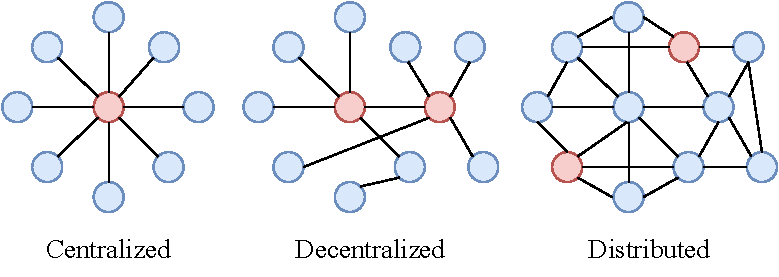
\includegraphics[width=0.8\linewidth]{obrazky-figures/DistributedSystemsComparison.pdf}
	\caption{Overview of distributed network architectures.}
	\label{DistributedSystemsComparison}
\end{figure*}

\noindent Figure \ref{DistributedSystemsComparison} visualizes the differences between the network architectures. In a centralized system, there is a single node (red color) with authority connected with all the other nodes (blue nodes). In decentralized systems, there is no single authoritative node. In distributed systems, each node in the system can be interconnected. The blockchain network is designed to be decentralized, as it is not maintained by a single controlling entity, but rather by a group of peers. 

\subsection{Blockchain}
\label{blockchain}
Blockchain is a distributed ledger or linked data structure replicated and distributed over a peer-to-peer network connected in a private, secure, and independent manner \cite{BeyondBitcoin}. The block structure consists of two parts: the block header and the block itself. The block contains ordered data, called transactions, placed into time-stamped blocks by achieving distributed consensus among the participants of the system. Each participating peer on the network validates transactions and keeps a copy of the blockchain. Consensus is an algorithm or mechanism that governs the behavior of the distributed system to remain correct. Bitcoin's ``Proof of Work''(PoW) protocol is among the most popular, where nodes follow an algorithm that uses computation power to calculate the hash value of a newly composed block until a target value is reached. Then the whole network can verify the block and reach an agreement. Other examples of consensus mechanisms are the Proof of Stake (PoS), Proof of Authority (PoA), and Proof of Elapsed Time (PoET). \cite{ConsensusInTheWild}. Transaction records can be of various types: currency transactions, health data, system logs, or traffic information \cite{HybridBlockchainIdentityAuthentication}. 

\begin{figure*}[h]
	\centering
	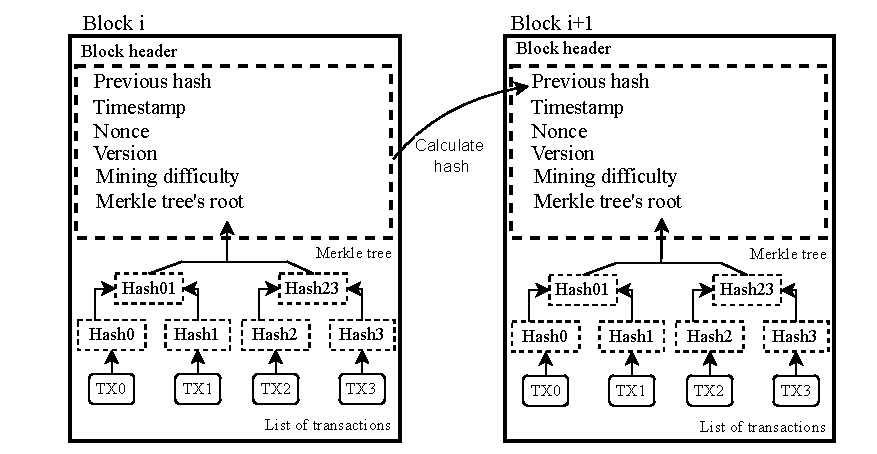
\includegraphics[width=\linewidth]{obrazky-figures/BlockchainArchitecture.pdf}
	\caption{Block structure in ``Proof of work'' blockchains.}
	\label{BlockchainArchitecture}
\end{figure*}

A list of transactions collected into the so-called ``blocks'' is bundled together, and each is stored as a hash. The block header is made public and accessible to anyone. In blockchains with a proof of work, the consensus mechanism block header contains two sets of metadata(see Figure \ref{BlockchainArchitecture}). One is associated with mining and is composed of timestamps, mining difficulty target, and ``nonce''. The second, associated with the block itself, consists of the hash of the previous block, the current version, and the Merkle tree root\cite{BeyondBitcoin}. Merkle tree is a tree of hash values of transactions (Merkle tree leaves), and the leaves are linked into a tree structure by recursive calculation of hashes of two adjacent transactions stored in the block until there is only one left (Merkle tree root). Each block in the chronological chain references the previous block by its cryptographic hash and every block validates transactions up to the present moment, so if the previous block is modified or not validated, any new block proposed to the existing chain gets rejected\cite{BeyondBitcoin}. This is the key factor in achieving the immutability and permanency of blockchains, which ensures the authenticity of data on the network and is one of the strongest characteristics of blockchain technologies. This means that modification of the data by an individual is very difficult. One would have to corrupt the majority of the nodes in the network to do so (e.g., in Bitcoin an individual would have to control 51\% of the computational power) \cite{MajorityIsNotEnough}. The blockchain network can be configured according to the use case and expected requirements in four categories \cite{BlockchainInOperationsManagement}: public blockchains, private blockchains, consortium blockchains, and hybrid blockchains.


%%The most popular application of blockchain technology is Bitcoin, the decentralized peer-to-peer cryptocurrency.
\subsubsection{Public blockchains}
Most popular cryptocurrencies, including Bitcoin and Ethereum, are public blockchains. Sometimes they are referred to as ``Permissionless blockchains'' since anyone without permission can access the blockchain network and become an authorized peer, trade monetary value, participate in consensus and ``write” to the shared state by invoking new transactions\cite{ConsensusInTheWild}. Therefore, a user or node can view all current or past records, examine executed computations, verify transactions, and participate in finding consensus among peers for the new incoming block. As a result, the blockchain is a self-governed network that encourages peers to join and participate. These networks operate an incentive scheme that rewards the participating nodes in return.

\subsubsection{Private blockchain}

Some organizations may not be interested in sharing their confidential information (for example, sensitive records in private blockchain healthcare applications\cite{blockchainInHealthcare}) with anyone on the Internet, but at the same time they still want to collaborate and share data. They are controlled by a single authority, so they are also referred to as ``permissioned blockchains'', since in this type of blockchain network only a limited number of peers can participate and be authorized. In this way, the information transmitted through the private blockchain stays within the network. Private blockchains are more centralized due to the limited group of participants. They are usually used in applications where the participating users must be fully identified and trusted. Examples of such a blockchain are Ripple (XRP) and Hyperledger\cite{ConsensusInTheWild}.

\subsubsection{Consortium blockchain}

Consortium blockchains are sometimes considered an intermediate access control architecture between private and public blockchains. They are similar to the previous type of ``permissioned blockchains'', still relatively private with semi-decentralized architectures. But compared to private blockchains, the difference is that now there is a consortium of authoritative individuals instead of one authority. The usual elements of their application are businesses and financial scenarios with a limited number of participants. Examples of such blockchains are Tendermint, Quorum, and Multichain\cite{ConsensusInTheWild}.

\subsubsection{Hybrid blockchain}

Hybrid blockchains are a unique type of blockchain that combines the best parts of private and public blockchain architectures. The right combination of the private and public blockchain protocol can optimize system throughput, latency, and scalability \cite{HybridPoSPBFT}.
They are flexible as they allow users to decide which information remains private and which information is made public. Compared to private blockchains, they are also not accessible to everyone, but features such as integrity, transparency, and increased security still remain.

\subsection{Smart contracts}
\label{Smart contracts}
The smart contract is essentially a piece of code written in Turing-complete language that runs in a secure environment (blockchain) that controls digital assets\cite{BlockchainAndBiometrics}. Many public blockchains support smart contracts, but the most widely used framework is Ethereum. Ethereum offers the possibility of writing your own smart contracts with its own high-level programming language. By sending transactions to the Ethereum network, users can create new contracts, request the execution of a certain function in a contract, or transfer digital assets (Eth in Ethereum) to other users or to other contracts. To guarantee the correct execution of smart contracts, each transaction is processed and resolved by the large pool of nodes running the ``Proof of Work'' consensus \cite{ConsensusInTheWild}. To send a transaction, the user must pay execution fees, which are paid to the nodes that run the consensus as an incentive to remain honest. This is one of the disadvantages of the Ethereum blockchain that its users must bear in mind.

\subsection{Practical byzantine fault tolerance}
Practical byzantine fault tolerance (PBFT) is a consensus algorithm that was developed to withstand Byzantine nodes (this comes from a family of Byzantine fault-tolerant protocols) in a distributed network to ensure its integrity \cite{PBFTCLassification}. Byzantine nodes are nodes that are faulty or subverted and intentionally respond with wrong decisions. All nodes must communicate and exchange messages until a two-thirds majority of votes is received, then the next block may be added. PBFT is a state machine replication algorithm that allows for the replication of complex operations over a network of clients with incorporated defense mechanisms against Byzantine faulty clients. 

The PBFT protocol consists of three phases: preprepare, prepare, and commit to \cite{PBFTAndProactiveRecovery}. Phases are needed to order requests sent in the same view or across views, even when the primary node is faulty. The protocol between four nodes with one of them being faulty is described in Figure \ref{PBFTDiagram}.
There are many alterations to this protocol that are being developed. Each is trying to optimize the original protocol in some aspects. For example, some works focus on structural optimizations that may introduce a hierarchical structure to the network \cite{PBFTCLassification}. Others are trying to simplify the overall process, for example, a work that incorporates reputation into the voting mechanism promises to reduce communication time, increase transaction throughput, and improve system efficiency and security \cite{ImprovedPBFTReputation}.

\begin{figure*}[h]
	\centering
	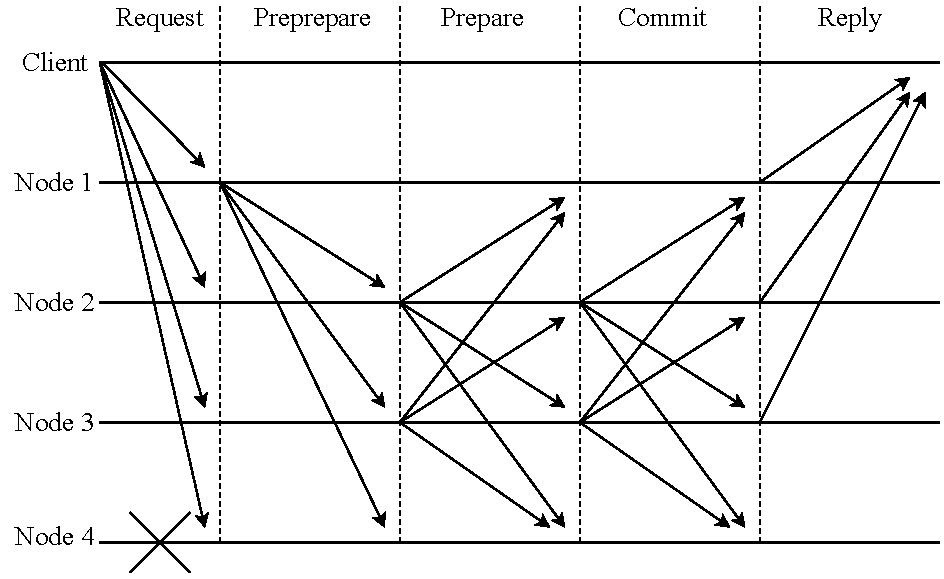
\includegraphics[width=0.9\linewidth]{obrazky-figures/PBFT.pdf}
	\caption{Practical byzantine fault tolerance architecture.}
	\label{PBFTDiagram}
\end{figure*}


The algorithm expects a minimal number of participating nodes $n$, as shown in Equation \ref{PBFTEquationMinParticipation}, where $f$ is the number of fault nodes, and $n$ is the number of all nodes in the network. Based on this equation, we can also derive the number of fault tolerant nodes $f$ (see Equation \ref{PBFTEquationFaultTolerance}) of the PBFT algorithm for the number of nodes $n$. \\

\newenvironment{conditions}
  {\par\vspace{\abovedisplayskip}\noindent\begin{tabular}{>{$}l<{$} @{${}={}$} l}}
  {\end{tabular}\par\vspace{\belowdisplayskip}}
  

\begin{equation}
        n = 3 f + 1
    \label{PBFTEquationMinParticipation}
\end{equation}
\begin{center}
    Number of Participating Nodes.
\end{center}

\begin{equation}
        f  = \frac{n - 1}{3} 
    \label{PBFTEquationFaultTolerance}
\end{equation}
\begin{center}
    Fault Tolerance.
\end{center}

where:
\begin{conditions}
 $n$     &  number of nodes in the system, where $n \in$ \mathbb{N}\\
 $f$     &  number of faulty nodes, where $f \in$ \mathbb{N}
\end{conditions}




\chapter{Design}
This chapter first analyzes existing consensus protocols and provides an overview of existing blockchain solutions for the security of biometric systems and explains the essential design principles of biometrics and blockchain. Subsequently, it describes the security of communication between nodes in the system. Finally, it introduces the proposed proof-of-concept design and demonstrates its functionality by describing scenarios of established biometric processes. 

\section{Consensus mechanism}
The selection of the consensus mechanism depends on the type of blockchain used. 
As stated in Section \ref{blockchain} above, there are four types of blockchain, each with its advantages and disadvantages. We needed to select one of them that best fits our proposed system. Table \ref{BlockchainTableTaxonomy} presents the categorization considered for our chosen consensus mechanism. 

\begin{table*}[h]
  \label{BlockchainTableTaxonomy}
  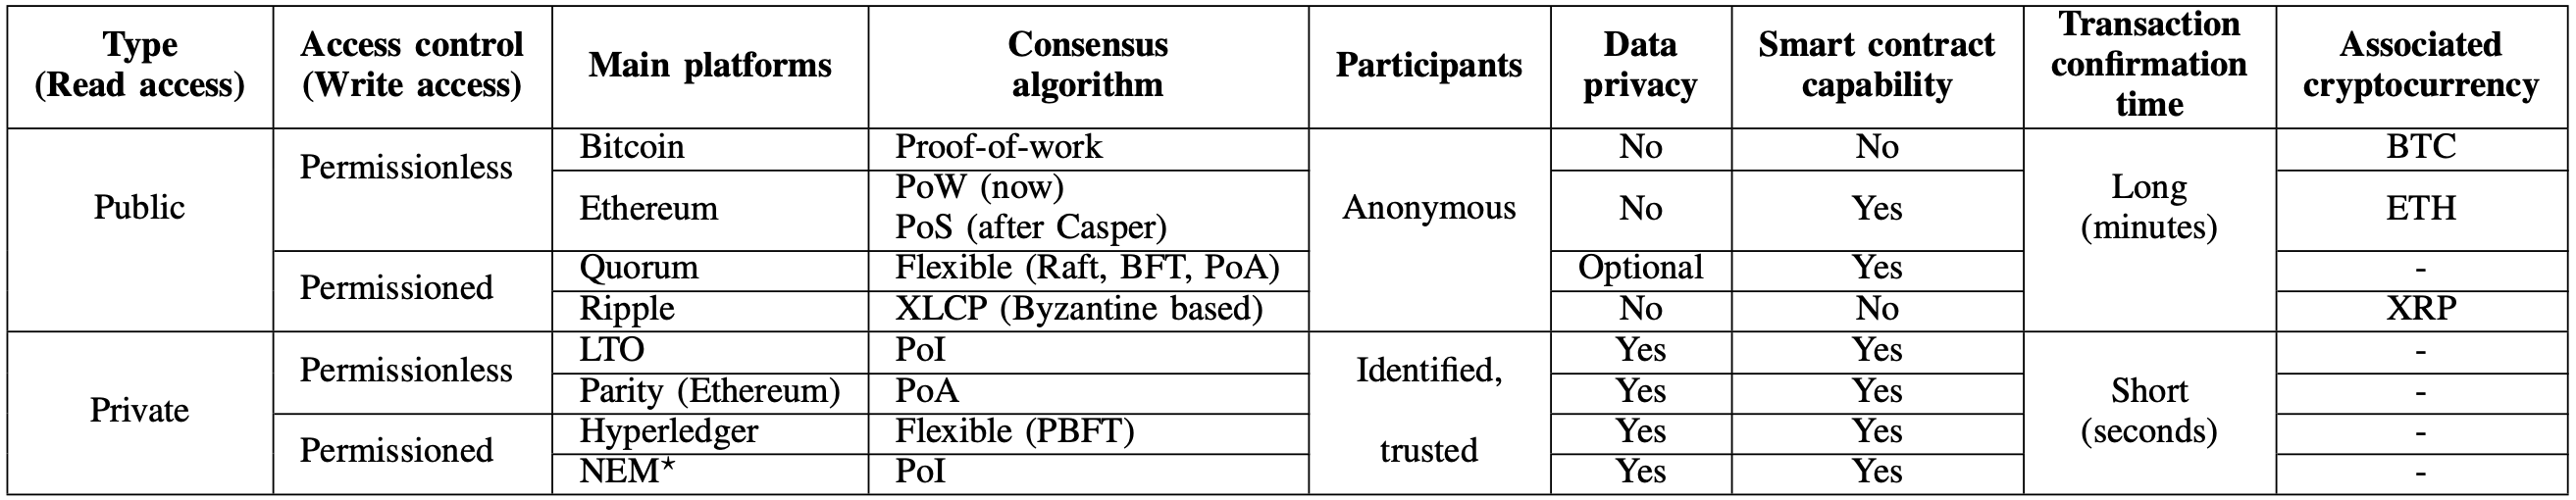
\includegraphics[width=\linewidth]{obrazky-figures/comparisonConsensus.png}
  \caption{Blockchain technology taxonomy \cite{BlockchainMeetsBiometrics}.}
\end{table*}

\subsection{Private vs public blockchain}
\label{Private vs public blockchain}
The first criterion that we must take into account is the privacy and accessibility of the system. We either might have the system publicly available for reading to anyone with Internet access by using the public blockchain, or we want to preserve the data by restricting access with the use of a private blockchain. We assume that the proposed system will be used within a single organization that demands private storage of their data, so the use of a private type of blockchain seems more fitting. By choosing a private blockchain, we also avoid the fees associated with the private blockchains (e.g., paying the gas fee for Ethereum transactions or execution of smart contracts).  But we lose on the higher level of security associated with public blockchains because, for example, the consensus that uses the mining process is much more robust against collusion attacks \cite{BlockchainMeetsBiometrics}.
Another criterion is the processing capacity and scalability. Private blockchains are typically much faster to process a transaction than public blockchains. For example, Ethereum can process only a dozen transactions per second compared to PBFT, where transactions have very high throughput and low latency. It is a great advantage of private blockchains, as the waiting time for transaction processing, for example, in Ethereum, is usually in the range of minutes \cite{ConsensusInTheWild}. This is a key factor for instant request-response-based systems, such as biometrics systems. Scalability is equally important. In public blockchains, all nodes must keep a copy of the blockchain. With each added block, the size of the blockchain increases (the size of the Ethereum and Bitcoin blockchains is hundreds of gigabytes \cite{BlockchainMeetsBiometrics}), which can be a problem for a variety of applications. From these criteria, we chose to design our system based on a private blockchain. Our system also assumes that the participating nodes are the terminals of the biometric authentication system. Therefore, every new terminal added must be controlled, trusted, and identified. Thus, we examine consensus protocols that utilize ``permissioned'' access control. 
\subsection{Private blockchain protocols}
\label{Private blockchain protocols}
Among the most prominent candidates for such protocols are Clique, Aura, PBFT, or its modifications (e.g., IPBFT \cite{ImprovedPBFTReputation}, weighted PBFT \cite{TacticalDatalinkPBFTWeighted}). All of these protocols are from a family of BFT protocols, which means that all of them can withstand subverted and faulty nodes. By choosing a protocol that tolerates subverted nodes, the proposed system addresses the single point of failure. In a recently published study \cite{CapTheoremPBFT}, these protocols were qualitatively compared applying the CAP theorem (in the distributed system only two of consistency, availability, and partition tolerance can be ensured at the same time), with results showing that the PBFT protocol maintains the blockchain consistent compared to Clique and Aura, where consistency was given up for availability. This means that PBFT makes it a priority to maintain the integrity of transactions. This is a desired characteristic for our use case, where the order of the transactions determines whether or not the user will be authenticated. PBFT is known for its high reliability, security, high throughput, and low latency \cite{PBFTCLassification}. Furthermore, it is feasible to implement the PBFT-based system from scratch. It comes at a cost that PBFT performs and scales slightly worse than its Clique and Aura counterparts, caused by its high communication overhead \cite{CapTheoremPBFT}. These drawbacks can be solved by using some alterations that improved, modified, and optimized some of these shortcomings. In our proposed system, we chose to work around PBFT due to the characteristics mentioned above and due to the possible future development allowed by extensive research on PBFT modifications aimed at optimization or extension of the system. Inspired by the work of blockchain-based data transmission control in tactical data link \cite{TacticalDatalinkPBFTWeighted}, we modified the classical PBFT, where each of the nodes is treated equally by introduction of weights into the system that allow customizability of trust in certain nodes.

\section{Weighted PBFT}
Modifying PBFT protocol with weights allows custom weight specification of the nodes in the system according to the probability that the node is compromised or defective. In practice, a biometric terminal close to the entrance of the building with access control and without many security mechanisms in place (e.g. camera, proper lightning, or security guard checks) would have a much higher probability of being attacked and compromised than a terminal in the center of the building with proper security mechanisms. Thus, the vote from the less secure terminal should have lower ``weight'' than the vote from the properly secured terminal.
The details and phases of the weighted PBFT protocol are described below.

\begin{figure*}[h]
	\centering
	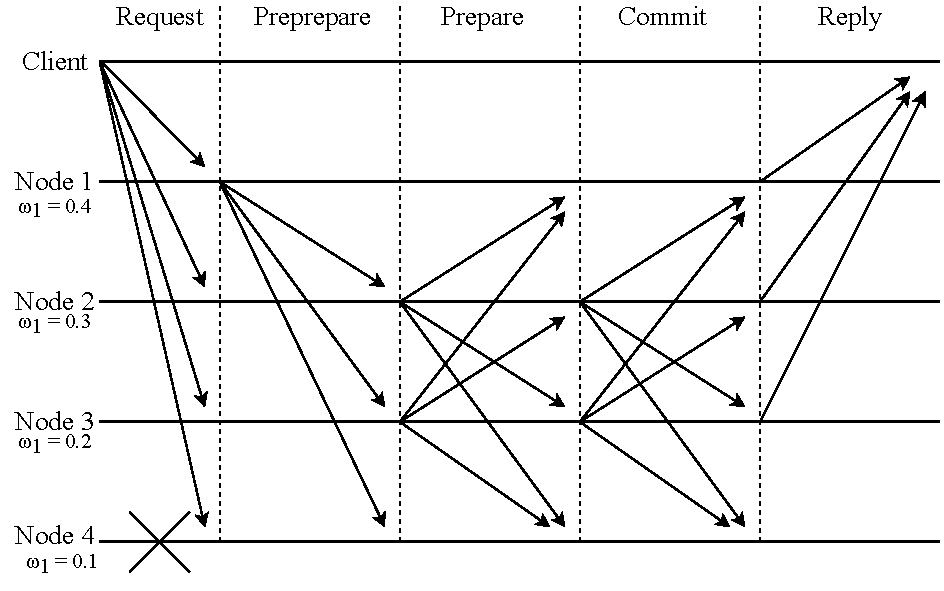
\includegraphics[width=0.8\linewidth]{obrazky-figures/WeightedPBFT.pdf}
	\caption{Weighted PBFT communication.}
	\label{WeightedPBFTcommunication}
\end{figure*}

\begin{enumerate}
    \item \textbf{Setup:} Here establishment of all parameters in the system is carried out, every node in the system generates its public/private key pair and gets its weight specified by the central authority in a way that corresponds to Equation \ref{WeightedPBFTEquationFaultSum}, where the sum of all the weights $\omega$ in the network of $N$ nodes equals one. Initially, the node with the highest weight is chosen as the primary node (see Node1 in Figure \ref{WeightedPBFTcommunication}).

    \begin{equation}
        \sum_{i=0}^{N} \omega_i = 1
        \label{WeightedPBFTEquationFaultSum}
    \end{equation}
    \begin{center}
        Network Weight Distribution
    \end{center}
    where:
    \begin{conditions}
     $N$     &  total number of nodes in the system, where $N \in \mathbb{N}$\\
     $\omega_i$     &  weight of a node with index $i$, where $i \in N$
    \end{conditions}
    
    \item \textbf{Request:} When node requests a block proposal or transaction validation, it first generates a signed request message that is transmitted to all consensus nodes. All nodes verify the signatures of that message and store it in their log. When the current primary node receives and verifies the request, it will also transmit a \emph{Preprepare} message to all the nodes. The \emph{Preprepare} message contains a hash value of the initial request and other values (view, sequence number) associated with the vote for a new primary node. 
    \item \textbf{Preprepare:}  Message and the validity of the sender node are verified, and the existence of the received hash value of the initial request is checked in the log. If everything is as expected, the \emph{Prepare} message is broadcasted.
    \item \textbf{Prepare:} Same process of conducting the verification of each message as previously is repeated again. Subsequently, the node in the \emph{Prepare} phase waits for the \emph{Prepare} messages received from the other nodes. For each node sender of the received \emph{Prepare} message, the node makes a request to the central authority that regulates the weights of the nodes. To broadcast the \emph{Commit} message and enter the \emph{Prepared} phase, the node waits until a sufficient number of \emph{Prepare} messages are received. The sufficient requirement is that the sum of the weights of the received \emph{Prepare} messages from network must be more then $\frac{2}{3}$, in accordance with Equation \ref{WeightedPBFTEquationNextPhaseSum}.
  
    \begin{equation}
        \sum_{j=0}^{N} \omega_{m_{j}} > \frac{2}{3}
        \label{WeightedPBFTEquationNextPhaseSum}
    \end{equation}
    \begin{center}
        Minimal Weight Threshold
    \end{center}
    where:
    \begin{conditions}
     $N$     &  total number of nodes in the system, where $N \in \mathbb{N}$\\
     $\omega_{m_{j}}$     &  weight $w$ of a message $m$ sent from $j$-th node, where $j \in N$ and $0\leq\omega_{m_{j}}\geq1$
    \end{conditions}
    
    \item \textbf{Commit:} Verification of the message and sender is executed again. The node waits and collects the \emhp{Commit} message until the sufficient weight according to Equation \ref{WeightedPBFTEquationNextPhaseSum} is reached. After reaching the \emhp{Committed} phase, the node is prepared to execute the requested operation (block proposal or transaction validation) from the locally stored data. Subsequently, the operation is executed, a \emph{Reply} message containing the result of the operation is constructed, and transmitted to the current primary node. In case the node does not reach sufficient weight in a certain time interval, the node does not transmit the \emph{Reply} message.
    \item \textbf{Reply:} Here primary node collects all the \emph{Reply} messages and waits until the weight threshold of Equation \ref{WeightedPBFTEquationNextPhaseSum} is reached again. When the primary node has enough \emph{Reply} messages, according to the agreement of the result, the operation is performed globally (e.g. storing template in database or adding block to the blockchain). 
\end{enumerate}

\section{Biometrics on blockchain}
\label{Biometrics on blockchain}
Blockchain offers characteristics such as immutability, auditability, availability, or universal access. These characteristics are desirable for biometric systems. Blockchain technologies require the distribution of data among peers participating in the network to achieve consensus. As a result of this single fact, it is important to follow the design convention when it comes to applying biometrics to the blockchain: \emph{``Biometrics, in its raw or derived form (templates), should never be stored(plain or encrypted) on a public distributed ledger system (such is blockchain).''}\cite{BiometricsOnBlockchain}. According to European regulations, it is even prohibited to store raw biometric data centrally (Regulation (EU) 2016/679\cite{EuropeanParliamentRegulation}), so distribution in the network is entirely out of the question. Encryption of stored templates is not the solution to this problem. There are no guarantees of safety and privacy for such data in the future (for instance, due to the rapid ongoing development of quantum computing).

Some works solved this with a segmentation mechanism that splits the templates into fragments, independently managed by each client. During authentication, this system runs a smart contract on a permissioned blockchain to find clients who manage the requested fragments\cite{SecuringBiometricAuthenticationBlockchain}. Others applied distributed identifiers or keys that are stored on a blockchain and also linked to a biometric template stored in the database \cite{BiometricsOnBlockchain}. Person biometrics remain privately stored in the secure database and the identifier / key is universally discoverable and reachable for biometric authentication. 

Since our work aims to secure the operation of certain components, resolving the issue with direct storage of biometrics on the blockchain through fragmentation could be excessive. The choice of identifier/key and biometric template pairs is more fitting. 

% TODO maybe do an image that showcases what is stored in the transaction in a block and showcase the reference to the database

\section{Securing the transmission}
Since the biometric data transmitted over the network is sensitive, it is necessary to encrypt them prior to transmission. The solution to this problem is to use hybrid cryptography. It combines the convenience of asymetric cryptography, where it is not required to share the same secret (key) in order to communicate securely, with symmetric cryptography, which is much more efficient in its computations. Many applications are avoiding asymetric cryptography, as its application on long messages causes high costs.
Participating nodes in the system are preauthorized by the central authority, and each assigned with a keypair of public and private keys. The nodes access the public keys from the central authority and use them to share symmetric key between node pairs. The messages exchanged between the nodes are then encrypted with the symmetric key.

% TODO try to implement the exchange of the symmetric keys with their private ones  and then you can describe it here, what kind of protocols wer used. Also mentioned the session key exchange ion PBFT protocol that refreshes the session keys every period or something
% x.509 certificate

\section{Description of the proposed system}
With the use of the PBFT protocol, the proposed system transforms the classical biometric system into a decentralized version with the incorporation of blockchain technology while performing biometric authentication operations. This extends the security mechanisms of classical biometric systems to make them more resilient to known issues such as a ``single point of failure'', the unreliability of the authentication process, and channel vulnerabilities against interceptions. Additionally, weights in the PBFT protocol allow for a custom distribution of voting power between nodes based on the security confidence of the given node. Organizations that will potentially apply the proposed system can customize it according to their needs and the security analysis of the environment in which the biometric system will be deployed. 
The goal of our design of the decentralized biometric system is to ensure that the matching and feature extraction components are not executed on their own. In addition, use the blockchain as an interface for the transmission of operational data, secure the communication ``channels'' connected with these components. 

Every process is identified with a universal unique identifier (UUID) \cite{UUIDCitation}, which is used to link the partial operations that make up the process. Since the results and metadata of the partial operations are stored on the blockchain in the form of transactions, this identifier enables the possibility to search for each operation that constitutes the given process. For example, to examine a failed process, it is possible to search for a given process UUID to see which of the particular operations has malfunctioned or got overridden. 

In our design, the template database remains centralized, where each template is paired with a key of a given user that is used as an identifier in the blockchain domain to meet the privacy requirements of sensitive biometric data. Each node keeps the received requests with the data in their logs, to be able to serve more requests at the same time. After a certain period of time passes, the given log is deleted. 

\begin{figure*}[h]
	\centering
	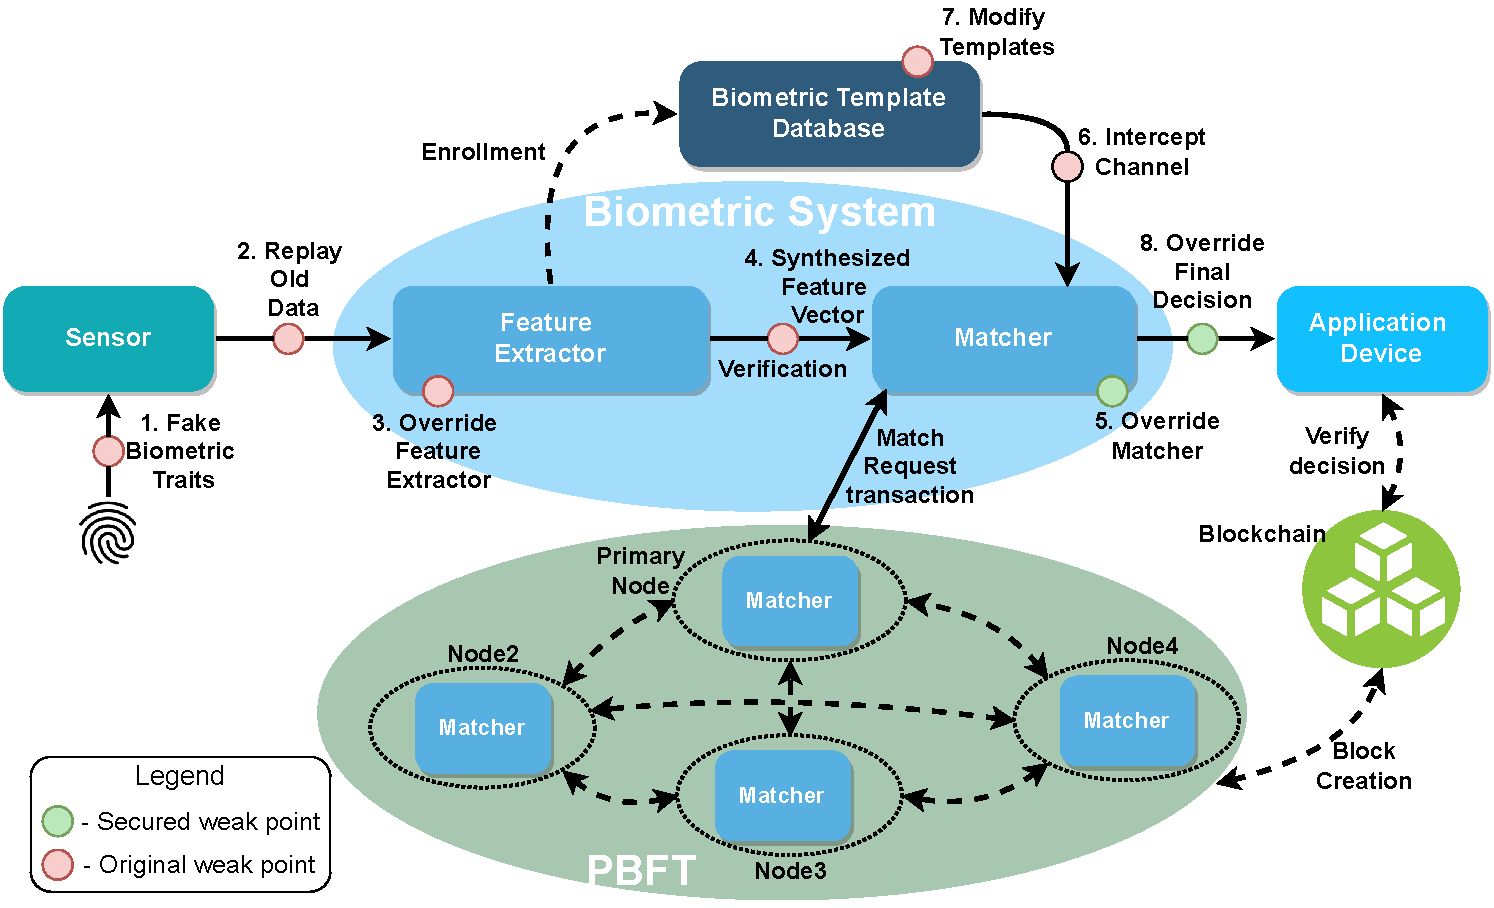
\includegraphics[width=\linewidth]{obrazky-figures/BiometricSystemIntegrationWithBlockchain.pdf}
	\caption{Incorporation of blockchain to biometrics in Matching component.}
	\label{BiometricSystemBlockchainDiagram}
\end{figure*}

Figure \ref{BiometricSystemBlockchainDiagram} presents a partial graphic representation of our proposed system, where the integration of the blockchain is shown only with the matching component. The red dots show the traditional weak points of the previous sections and the green dots show the weak points that are tackled with our design. The decentralized manner of execution of the matching operation secures weak point number five. The blockchain can also be used to inspect operations performed in the decentralized biometric system as a way to verify the final decision received in the external application, thus securing the weak point number eight as well. With similar principles, our design is also used to secure the feature extraction component.


\section{Scenarios of system's operation}
As previously mentioned in Section \ref{BiometricTypicalProcesses} the classical biometric systems usually perform enrollment, identification, and verification processes.
Their execution and the components responsible for their orchestration in a classical biometric system were described in \ref{BiometricModules}. For a better understanding of the inner functioning of the proposed system compared to the conventional biometric system, we describe our methodology behind each of these processes. 

% Our system assumes that the security against direct attacks on the sensor module is handled within the organizational procedures(e.g. supervised enrollment).
\subsection{Enrollment}
During enrollment the key objective is to register a new template record in the database. Figure \ref{PBFTSequenceDiagram} helps to understand the methodology by following the sequence diagram. For this process, the participation of the sensor and the feature extractor is required. At the initial point of authentication, the sensor module operates in a standard way, collecting the raw biometric data in a single terminal/node of the biometric system and converts and transmits them to the feature extraction module. After receiving the digital biometric data, the feature extractor processes the data to form them into a template.
\begin{figure*}[h!]
	\centering
	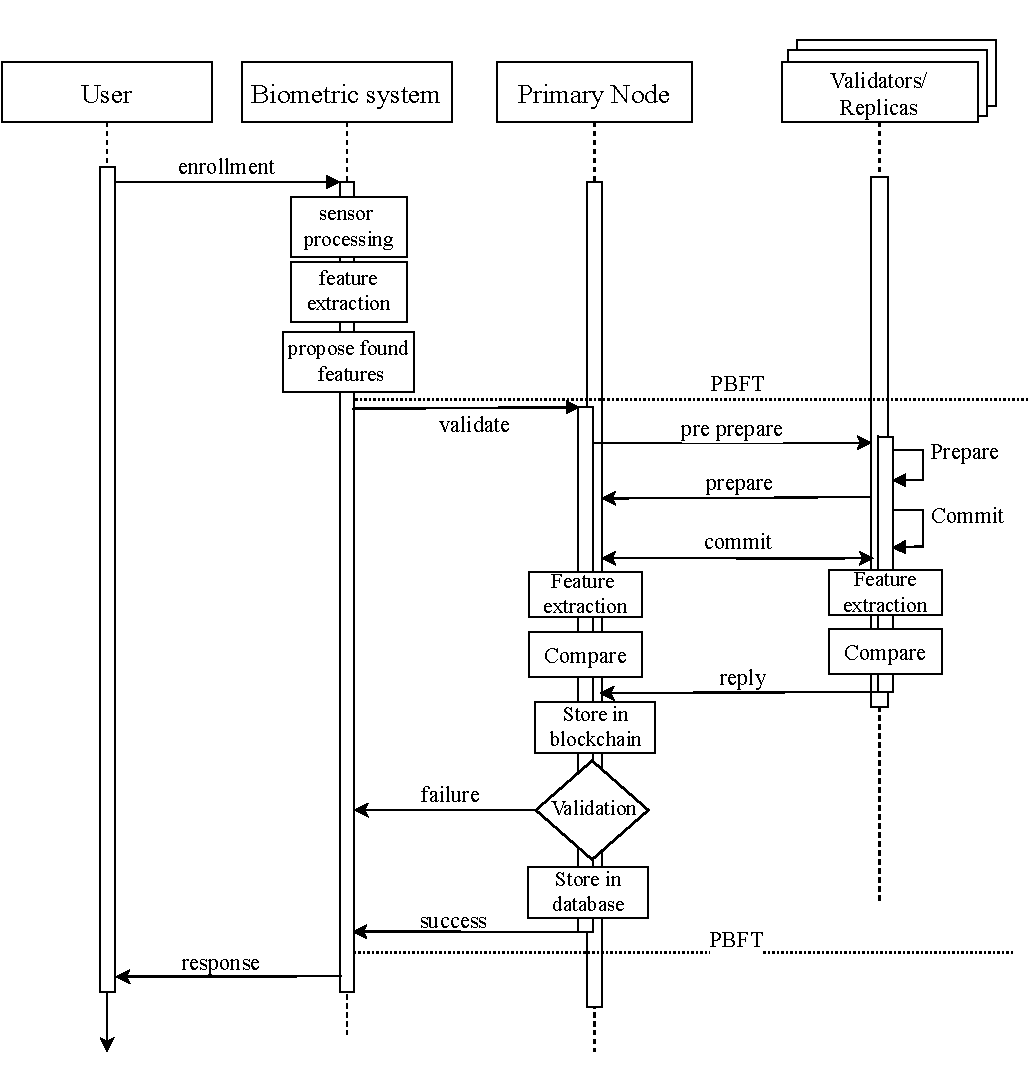
\includegraphics[width=\linewidth]{obrazky-figures/SequenceDiagramFeatureExtract.pdf}
	\caption{Communication in proccess of feature extraction during enrollment.}
	\label{PBFTSequenceDiagram}
\end{figure*}

The security of feature extraction is already included in our proposed system design. Its execution may end in success or failure. Therefore, the template is not stored in the template database, or the user is not asked to repeat the biometrics collection immediately, as would be the case in the classical biometric system. Both outcomes will first be validated in the distributed network of authorized nodes. After feature extraction's classical operation, two data collections are assembled: the operational data (transaction) about the feature extraction (outcome, timestamps, etc.), and the sensitive data (biometrics and the extracted template). The node requests validation of its feature extraction and transmits a message with the beforementioned data collections over encrypted channels to other nodes in the network. All receiving nodes verify this message and store the data in their log. When the primary node in the PBFT protocol receives the request message, it starts a new round of the PBFT protocol. Here, the nodes exchange messages and verify the operation by executing it with the request data in their log and comparing it with the data stored inside the transaction. The result of the comparison is then transmitted to the primary node. After the primary node receives enough replies and the validation result was positive, it stores the template paired with the user identifier from the transaction in the database and the transaction into the local queue. Furthermore, if the transactions in the queue reach a threshold or timeout, the primary node proposes a new block containing the transactions that will be added to the blockchain and must be agreed upon by the network, according to the PBFT protocol. When the block is proposed and added to the blockchain, all transactions contained in this block are deleted from the log.
\subsection{Identification and Verification}
In this two scenarios, additionally to the feature extraction, it is required to perform a comparison with the templates stored in the template database. The feature extraction is performed as in the enrollment scenario. After receiving the template from feature extraction, the blockchain is searched for the transaction of the current identification/verification process, and the result is inspected. If the feature extraction operation was successful, matching can be performed. The matching of the templates is executed, and the data split into two collections again, with the exception that sensitive data now hold only compared template and the operational data in addition contain user identifier that corresponds to the matched template. The node assesses the blockchain to determine whether the feature extraction was previously performed successfully. If the assessment was positive, the node requests validation of the performed matching over encrypted channels to other nodes, where the matching is performed and validated. Each node first examines the blockchain for a successful prerequisite feature extraction and performs the matching. In case of positive matching of the templates, the identifier of the matched user is compared with the identifier received in the transaction identifier. The result is transmitted again to the primary node. In the event of enough positive validation responses, the user is successfully identified/verified. The transaction for matching validation request is stored again in queue and waits for the block proposal.

%TODO možno by sa to checklo zmieniť že tie public kluče pre vymenu sprav by boli spravovane nejakou centralnou autoritou u nas bioblockchain module

\chapter{Implementation}
This chapter describes the details of the implementation of the demonstrator program, shows its representative architecture, and describes the role of each module (see Figure \ref{DependencyArchitecture}).
All modules of the program are implemented in Python language and are documentated dynamically by the Sphinx library, which generates webpages from annotated comments of given classes, functions, or variables. This choice of technologies allows for ease of implementation for the proof-of-concept demonstrator of messages in the proposed system. All modules are written from scratch, using only publicly available standard, cryptographic, or asynchrounous libraries. For ease of use and to guarantee correct versions of the libraries, the program was developed using a virtual environment, and all required libraries are specified in \texttt{requirements.txt}.
\begin{figure*}[h]
	\centering
	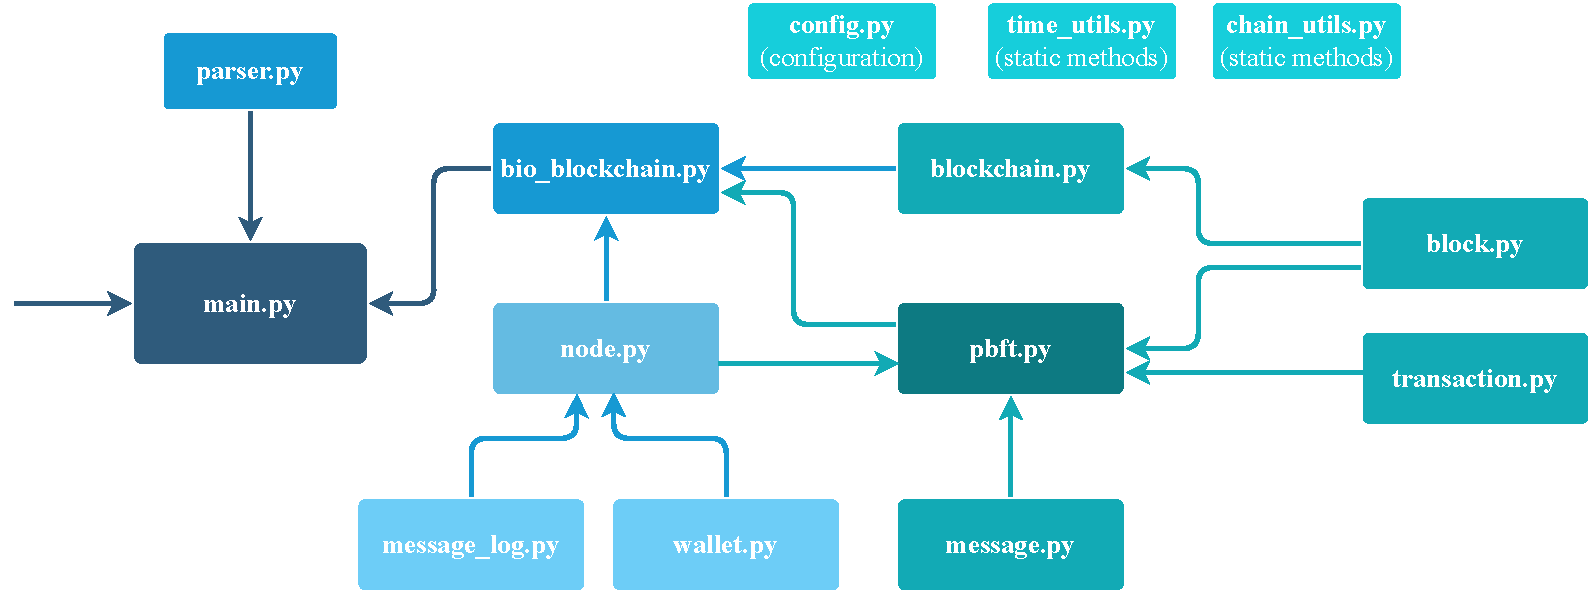
\includegraphics[width=\linewidth]{obrazky-figures/DependencyArchitecture.pdf}
	\caption{Dependecy architecture of the demonstrator proof-of-concept program.}
	\label{DependencyArchitecture}
\end{figure*}
\section{Main module}
\label{Main module}
The \texttt{main.py} module orchestrates the execution of the demonstration scenarios in the \emhp{bioblockchain} program. Firstly, it instantiates the \emph{Parser} class that processes the passed arguments and on their basis determines the execution scenario of the simulator to be demonstrated. Within the demonstration program, we implemented five scenarios. Each can be invoked by its corresponding argument. Additionally, the demonstrator program supports a verbose mode that gives more information about the communication and the data stored in the system. Arguments from given scenarios are not combinable. Only combinations of verbose mode and a certain scenario are allowed. Without specifying the arguments, the program's default phase of operation is the successful enrollment of a new user and his subsequent verification and identification. The list of all supported arguments is as follows.
\begin{itemize}
    \item \texttt{Help (-h)} - Provides information on the options to run the demonstrator program. 
    \item \texttt{Verbose (--v)} - Provides extended information on network communication and makes it possible to view the contents of the blockchain or the template database after running a certain scenario.
    \item \texttt{Unknown individual verification (-uiv)} - Demonstrates a scenario in which an unknown individual claims to be verified as someone known to the system.
    \item \texttt{Unknown individual identification (-uii)} - Demonstrates a scenario of identification of an individual who is unknown to the system.
    \item \texttt{Feature extraction malfunctioned (-fem)} - Demonstrates a scenario in which feature extraction was compromised by an adversary who modified the extracted template in a way he has chosen.
    \item \texttt{Node malfunction returns always true (-nmat)} - Demonstrates a scenario in which one of the nodes in the network is compromised or malfunctioning and always returns a positive response to the request.
    \item \texttt{Node malfunction return always false (-nmaf)} - Opposite scenario to the previous, now one of the nodes in the network is compromised or malfunctioned and always returns a negative response.
    \item \texttt{Feature extraction and matcher channel interception (-femi)} - In this scenario the attacker intercepted the channel between the matcher and the feature extraction module and attempted to replay the captured data of the legitimate user to the matcher module, with the goal of authenticating himself.

\end{itemize}
\section{Biometric system's operation}
It is handled with the \emhp{BioBlockchain} and \emhp{Node} modules. The module \texttt{Node} represents a single terminal/node in the system and contains methods that simulate the operation of standard modules in the biometric system \ref{BiometricModules}. 
The \emhp{BioBlockchain} is a container or interface of the proposed system. It contains a list of all nodes participating in the network, its primary template database, and the blockchain. The list of nodes or network is set up according to the \texttt{NUM\_PARTICIPATING\_NODES} variable in \texttt{config.py}. Variables such as weigh threshold or number of fault tolerance calculated from Equation \ref{PBFTEquationFaultTolerance} are specified here as well. 

According to the scenario specified in the main module, the corresponding calls are made to the class methods of \emhp{BioBlockchain}. At first, a node in the network is randomly selected using the \texttt{get\_random\_node} method. This node represents a single terminal that was approached to perform biometric authentication / enrollment as described in Section \ref{BiometricTypicalProcesses}. In addition to that, the \emhp{BioBlockchain} class implements two methods, each simulating a standard biometric process of:
\begin{description}
    \item \textbf{Enrollment} (\texttt{run\_enrollment}) - manages the standard operation of the enrollment process in the proposed system. It starts by identifying the process with UUID, retrieved from the static method \texttt{ChainUtils.id} with the use of the \texttt{uuid} standard library. Then the acquisition of biometrics through the sensor is simulated using the \texttt{get\_sensor\_data} method of the randomly selected terminal/node. For the purposes of the demonstator, the biometric collection is simplified to the generation of hashes with \texttt{MD5} from \texttt{hashlib}. The hash is returned and passed to \texttt{feature\_extractor}. Here, extraction is performed with the \texttt{MD5} hashing function in a similar way as before. In this way, the same hash (``template'') is generated from the same input (``biometrics''), thus it is possible to simulate successful feature extraction. Afterward, the method creates two data dictionaries: sensitive data with biometric data paired with the extracted template and operational data. The contents of the operational data are shown in the Listing \ref{FeatureExtractionEnrollmentData}. In addition to basic information on the execution of the feature extraction and the outcome, the operational data dictionary also contains the identifier of a ``user'' who is enrolled. These dictionaries are passed to the \texttt{validate\_decision} method of the \texttt{pbft.py} module, where the data will be evaluated in the distributed network of nodes and eventually the operational data will be stored on the blockchain. In case of successful validation, the extracted template will be stored in the template database as a pair of user's identifier and the extracted template.
    \begin{lstlisting}[language=json,frame=single,breaklines=true, caption={Transaction data of feature extraction in enrollment.},captionpos=b, label={FeatureExtractionEnrollmentData}]
     "data": {
        "approached_node": "NODE2",
        "match_timestamp": "12.07.1999",
        "operation": "Feature Extraction",
        "process_id": "ef41d358-0617-11ed-a56b-8c85906ae247",
        "process_type": "enrollment",
        "success": true,
        "user": "6c18ffb87da096bb36fb5b58450e0efa33e0b49e9e0d552f0bad"
    },
    \end{lstlisting}
    \item \textbf{Authentication} (\texttt{run\_authentication}) - This method simulates both identification and verification depending on the passed \texttt{process} argument. For verification, it is also required to pass an argument with \texttt{claimed\_identity}. The initial phase of the authentication process (feature extraction) remains the same as in enrollment. After the network in the \texttt{PBFT} module reaches consensus and stores the result of the feature extraction operation on the blockchain, the data matching can be performed with the node's \texttt{matcher} method. Here, depending on the type of process, the extracted template is compared with every template stored in the database (identification) with the \texttt{features\_in\_database} method, or only compared to the claimed identity (verification) with the \texttt{claimed\_identity\_in\_database} method. The result of this comparison is the user identifier or \texttt{None}. Here again, all operational data is saved in a dictionary shown in Listing \ref{MatchingIdentificationData}. The template and operational data are then passed to \texttt{validate\_decision}, where the matching result will be evaluated and the operational data will be stored on the blockchain.
    \newpage
    \begin{lstlisting}[language=json,frame=single,breaklines=true, caption={Transaction data of feature extraction in enrollment.},captionpos=b, label={MatchingIdentificationData}]
    "data": {
        "approached_node": "NODE2",
        "match_timestamp": "12.07.1999",
        "operation": "Matching",
        "process_id": "295cee12-068e-11ed-82c8-8c85906ae247",
        "process_type": "identification",
        "score": 87,
        "success": true,
        "user": "6c18ffb87da096bb36fb5b58450e0efa33e0b49e9e0d552f0bad"
    },
    \end{lstlisting}
\end{description}
\section{Cryptographic operations}
\label{Cryptographic operations}
Cryptographic functionalities are implemented with the easy-to-use Python library \texttt{ecdsa} that supports the creation of key pairs (signing / private key and verifying / public key) and with the Python standard library \texttt{hashlib} that provides a common interface to many different secure hash and message digest algorithms. All cryptographic operations are implemented statically in the \texttt{ChainUtils} module. The proof-of-concept program does not contain an implementation of hybrid cryptography, that was described in design, all the exchanged messages are encrypted only with the use of asymmetric cryptography.

\subsection{Wallet}
This module is the foundation for most of the cryptographic mechanisms implemented in the program. It contains two parameters that store the public and/or private keys of some entity in the system (the nodes participating in the network or enrolled users in the biometric system). The private key / signing is acquired from a static function \texttt{generate\_key\_from\_seed} that takes a certain \texttt{seed} as argument. The seed is needed to generate a secret exponent \texttt{secexp} by calling a \texttt{randrange\_from\_seed\_trytryagain} method with two arguments: the seed and the \texttt{NIST256p} curve used to generate the secret exponent. Subsequently, the secret exponent is used to instantiate a \texttt{SigningKey} class by invoking the method \texttt{from\_secret\_exponent}. The \texttt{SigningKey} class then allows the creation of the associated \texttt{VerifyingKey} that is used to verify the signatures made by the \texttt{SigningKey}. Data signing is performed in \texttt{ChainUtils.sign}. To sign the data we need its digital hash digest representation. The hash digests are calculated in \texttt{ChainUtils.hash} with the \texttt{sha256} method from \texttt{hashlib}. The data signature is then obtained with the \texttt{SigningKey}s method \texttt{sign\_digest\_deterministic}. Verification of signatures is done using the static method \texttt{ChainUtils.verify\_signature}. This method takes two arguments: signed data, signature, and verifying key. The signed data must first be converted to the \texttt{bytes} data type. Subsequently, the previously created \texttt{VerifyingKey} provides a method for verifying the signature of the given data. 
\subsection{Blockchain and transactions}
The \texttt{Blockchain} class has a list of blocks and provides methods for the creation, verification, and addition of blocks to the blockchain. Since blocks are cryptographically bound together, the blockchain is initialized with the genesis block. The \texttt{Block} class represents a single block on the blockchain, each having its own hash value, hash of the previous block, the proposer's public key, signature, data/transactions payload, and other accompanying information (see Listing \ref{BlockchainData}). All cryptographic operations are implemented using methods previously described in Section \ref{Cryptographic operations}, and timestamps are acquired with the library \texttt{datetime}.
\begin{lstlisting}[language=json,frame=single,breaklines=false, caption={Two blocks chained together to form blockchain.},captionpos=b, label={BlockchainData}]
- - - - - - - - - - - - - - - - - Block - - - - - - - - - - - - - - - - -
Timestamp   : 18/06/2022 16:16:18
Last Hash   : dda9024382573e0a13da84e1e2f3ab7d5a614296ad3edeb79b2a4c366abe
Hash        : f513c5701029be442c24035b9c210a2d594f5ee245d4ee7c98902a76ca05
Data        : "Genesis"
Proposer    : 54bffd9ef9cf0a1a7d013b476c558e466cc73cc
Signature   : 0a473767eea58c61b0e4e66969c26b9e8068b7d3fe141
Sequence No : 1
- - - - - - - - - - - - - - - - - - - - - - - - - - -- - - - - - - - - - -
        
- - - - - - - - - - - - - - - - - Block - - - - - - - - - - - - - - - - - -
Timestamp   : 18/06/2022 16:16:18
Last Hash   : f513c5701029be442c24035b9c210a2d594f5ee245d4ee7c98902a76ca05
Hash        : 27176b5db0c16c9acc0f177592ca0fc664a9f19a0d7a9e70d906a5cbc45d
Data        : Transactions
Proposer    : 54bffd9ef9cf0a1a7d013b476c558e466cc73cc
Signature   : a45c55478caa1d993848d48d85d85a66b34e8d9e944bb
Sequence No : 2
- - - - - - - - - - - - - - - - - - - - - - - - - - -- - - - - - - - - - - 
\end{lstlisting}

Each transaction in the system is represented by the \texttt{Transaction} class. Transactions have parameters and methods similar to those of the \texttt{Block} class. With one exception, the absence of a hash reference to the previous transactions.

\section{Consensus system}
The orchestration of communication between nodes that try to reach consensus is handled in the \texttt{PBFT} class with the transmission of messages represented in the \texttt{Message} class. Messages exchanged in the original protocol are asynchronous. Therefore, we use an asynchronous Python library \texttt{asyncio} that allows for a more accurate simulation of communication in the demonstrator program. The proof-of-concept implementation of the system does not contain all the mechanisms (view changes, key exchanges) in the PBFT protocol.

Every message exchanged in the protocol is first verified, and then, depending on the phase, certain operations are performed. Round of consensus starts in \texttt{validate\_decision} or \texttt{validate\_block}. Here, the transaction or block is constructed and subsequently transmitted to other nodes with a validation \emph{Request} message.
The receiving node verifies the content transmitted in the \emph{Request} message and stores the hash value of the message in the log of the given node as a pair with the message contents. If the node that received the request message is primary, it transmits the \emph{Preprepare} message, containing the hash value of the initial request, to other nodes and begins another phase.

After the node has received the \emph{Preprepare} message, it inspects if the received hash value is already stored in its log. Subsequently, it transmits a \emph{Prepare} message containing the hash value of the request to other nodes. Every node that receives the \emph{Prepare} message increases the corresponding counter until a threshold from Equation \ref{WeightedPBFTEquationNextPhaseSum} is reached. Then sends a \emph{Commit} message using the \texttt{broadcast\_commit} method.

In the \emph{Commit} phase, the nodes increase the counter of the received \emph{Commit} messages. When the threshold is reached again, the operation is performed and verified using the \texttt{verify\_block} or \texttt{verify\_decision} method.  The result of the validation and the hash of the original request are composed of the \emph{Reply} message and transmitted to the primary node.

The \emph{Reply} phase consists of collecting validation results until the threshold of Equation \ref{WeightedPBFTEquationNextPhaseSum} is reached again and, based on those results, execute the given operation. The execution of the operation is performed using the \texttt{execute\_operation} method. Here, the primary node, depending on the request, either stores the template into the database or adds a new block to the blockchain. The network may instead of agreeing on the proposed request, agree on a different result (for example, the proposed extracted template for given biometrics is artificially produced, and the system agreed on a legitimate template).


\chapter{Evaluation and testing}
 Firstly this chapter tests the behavior of the implemented system's demonstrator by executing prepared scenarios of successful or unsuccessful execution. Then based on these scenario results and the presumed effect of our design, we evaluate the security of the proposed system, deciding which weak points are addressed and which are still present, what did the system solve and what are the drawbacks the system still suffers with. 
\section{Testing scenarios}
Within each testing scenario, the system is first set up according to the settings specified in the configuration file. Then the given scenario is performed, and the program shows the communication and the result of the system. All scenarios are available to be demonstrated in our program, by passing the arguments specified in Section \ref{Main module}.
The purpose of the given scenarios is to demonstrate the decentralized manner of the proposed biometric system and its ability to function under expected and also malicious conditions. For ease of demonstration purposes, the system is configured to consist of four nodes, where each node has the same weight. The following listings in testing scenarios do not contain the whole output of the program but just a key part of them.
\subsection{Expected behavior}
This scenario tests the system on the expected and successful execution of the enrollment process and its subsequent authentication of the enrolled user. For enrollment to proceed, present administrator must be authenticated first. The single node approached by the user in this test is honest, so requests for validation of the executed feature extraction are agreed upon (see Listing \ref{EnrollmentSuccesTerminalOutput}). After transmitting the request to the network and enough nodes respond with a successful response, the primary node successfully stores the extracted template in the database. Afterwards, the enrolled user tries to authenticate himself. Again, the honest node validation request is agreed upon (see \ref{VerificationSuccesTerminalOutput}) and the user is authenticated.

\lstset{escapeinside={<@}{@>}}

\newpage
\begin{lstlisting}[language=bash, frame=single, caption={Terminal output for enrollment.},captionpos=b, label={EnrollmentSuccesTerminalOutput}]
- Sensor scanning raw biometrics...
- Feature extractor processing raw data...
- Extracted features requesting to be validated...
<@\textcolor{Green}{- Creating new request for extraction validation of SUCCESS enrollment!}@>
--------------------------------PBFT START---------------------------------
<@\textcolor{Aquamarine}{- NODE2			 executing feature extraction}@>
<@\textcolor{Green}{- NODE2 		 validated!, sending "REPLY" message!}@>
<@\textcolor{Aquamarine}{- NODE0			 executing feature extraction}@>
<@\textcolor{Green}{- NODE0 		 validated!, sending "REPLY" message!}@>
<@\textcolor{Aquamarine}{- NODE1			 executing feature extraction}@>
<@\textcolor{Green}{- NODE1 		 validated!, sending "REPLY" message!}@>
<@\textcolor{Green}{- Enough replies have been received!}@>
<@\colorbox{Green!30}{- Feature extraction result has been validated!}@>
<@\colorbox{Green!30}{- Storing features into database!}@>
<@\textcolor{Aquamarine}{- NODE3			 executing feature extraction}@>
<@\textcolor{Green}{- NODE3 		 validated!, sending "REPLY" message!}@>
---------------------------------PBFT END----------------------------------
\end{lstlisting}

\begin{lstlisting}[language=bash,frame=single,breaklines={false}, caption={Terminal output for verification.},captionpos=b, label={VerificationSuccesTerminalOutput}]
<@\textcolor{Green}{- Creating new request for extraction validation of SUCCESS verification!}@>
--------------------------------PBFT START---------------------------------
<@\textcolor{Aquamarine}{- NODE2			 executing matching verification}@>
<@\textcolor{Green}{- NODE2 		 validated!, sending "REPLY" message!}@>
<@\textcolor{Aquamarine}{- NODE0			 executing matching verification}@>
<@\textcolor{Green}{- NODE0 		 validated!, sending "REPLY" message!}@>
<@\textcolor{Aquamarine}{- NODE1			 executing matching verification}@>
<@\textcolor{Green}{- NODE1 		     validated!, sending "REPLY" message!}@>
<@\textcolor{Green}{- Enough replies have been received!}@>
<@\colorbox{Green!30}{- Matching result has been validated, successfull verification!}@>
<@\textcolor{Aquamarine}{- NODE3			 executing matching verification}@>
<@\textcolor{Green}{- NODE3 		 validated!, sending "REPLY" message!}@>
---------------------------------PBFT END----------------------------------
\end{lstlisting}

\subsection{Unknown user authentication or identification}
\label{Unknown user authentication or identification}
Here, the testing scenario consists of a successful execution of the enrollment process and a subsequent malicious attempt to authenticate an unknown attacker who has overridden the matching module in a single node. Validation of feature extraction in both the enrollment and authentication process is successful (as seen in \ref{EnrollmentSuccesTerminalOutput}). In the authentication process, in which the compromised matcher component participates, the attacker attempts to verify himself as a previously enrolled user by overriding the matching decision. Hovewer, the request for the validation of the positive authentication to the network is disagreed on, and the outcome on the majority of the peers is different (see Listing \ref{MatchingFailTerminalOutput}). The network concluded that the request was a failed verification, thus the attacker's attempt to impersonate the enrolled user was unsuccessful. A similar scenario would occur in identification, where the unknown attacker would attempt to successfully identify himself as someone known to the system.
\begin{lstlisting}[language=bash, frame=single, caption={Terminal output for failed verification.},captionpos=b, label={MatchingFailTerminalOutput}]
<@\textcolor{Green}{- Creating new request for matching validation of SUCCESS verification!}@>
--------------------------------PBFT START---------------------------------
<@\textcolor{Aquamarine}{- NODE2			 executing matching verification}@>
<@\textcolor{red}{- NODE2 		 failed validation!, sending "REPLY" message!}@>
<@\textcolor{Aquamarine}{- NODE0			 executing matching verification}@>
<@\textcolor{Green}{- NODE0 		 validated!, sending "REPLY" message!}@>
<@\textcolor{Aquamarine}{- NODE1			 executing matching verification}@>
<@\textcolor{red}{- NODE1 		 failed validation!, sending "REPLY" message!}@>
<@\textcolor{Aquamarine}{- NODE3			 executing matching verification}@>
<@\textcolor{red}{- NODE3 		 failed validation!, sending "REPLY" message!}@>
<@\textcolor{Green}{- Enough replies have been received!}@>
<@\colorbox{Yellow!30}{- Verification result has been disagreed with, other outcome determined!}@>
---------------------------------PBFT END----------------------------------
\end{lstlisting}
\subsection{Feature extractor compromised}
\label{Feature extractor compromised}
Within this test scenario, the attacker compromised the feature extraction component in one of the nodes, with the intention of inserting his template within the honest enrollment of some user. During the enrollment of a legitimate enrollee, the feature extractor ignores received biometric raw data, and the attacker inserts his own template instead of producing a legitimate one. When the approached node requests validation of such extraction, to get them stored in the database. The rest of the nodes with the uncompromised feature extractor disagree and store a legitimate template extracted from the biometric data received from the legitimate enrollee. 
% An unsuccessful validation request is stored on the blockchain. 
%The system administrator or the person responsible for adjusting the weight nodes can review the blockchain, identify these attempts, and react accordingly (increase security mechanisms near the particular node or adjust the weight of the node).
\begin{lstlisting}[language=bash,frame=single,breaklines={true}, caption={Terminal output for enrollment from compromised node.},captionpos=b, label={EnrollmentCompromisedTerminalOutput}]
- Sensor scanning raw biometrics...
- Feature extractor processing raw data...
- Extracted features requesting to be validated...
<@\textcolor{Green}{- Creating new request for extraction validation of SUCCESS enrollment!}@>
--------------------------------PBFT START---------------------------------
<@\textcolor{Aquamarine}{- NODE2			 executing feature extraction}@>
<@\textcolor{red}{- NODE2 		 failed validation!, sending "REPLY" message!}@>
<@\textcolor{Aquamarine}{- NODE0			 executing feature extraction}@>
<@\textcolor{Green}{- NODE0 		 validated!, sending "REPLY" message!}@>
<@\textcolor{Aquamarine}{- NODE1			 executing feature extraction}@>
<@\textcolor{red}{- NODE1 		 failed validation!, sending "REPLY" message!}@>
<@\textcolor{Aquamarine}{- NODE3			 executing feature extraction}@>
<@\textcolor{red}{- NODE3 		 failed validation!, sending "REPLY" message!}@>
<@\textcolor{Green}{- Enough replies have been received!}@>
<@\colorbox{Yellow!30}{- Feature extraction result has been disagreed with, result determined!
}@>
<@\colorbox{Yellow!30}{- Storing features into database!}@>
---------------------------------PBFT END----------------------------------
\end{lstlisting}
\subsection{Node malfunction}
\label{Node malfunction}
In this scenario, a situation where one of the nodes on the network is defective and responds or proposes incorrect decisions. For example, in the case of enrollment, incorrect responses from the defective node have no effect on the result of feature extraction (see Listing \ref{NodeMalfunctionTerminalOutput}). When the decision is not unanimous, in order to ensure maximum safety, the system notifies the administrator or the weight management authority about the defective or malfunctioning node (similarly would be the case in other test scenarios).
\begin{lstlisting}[language=bash,frame=single,breaklines={false}, caption={Terminal output for enrollment with one malfunctioning node.},captionpos=b, label={NodeMalfunctionTerminalOutput}]
<@\textcolor{Green}{- Creating new request for extraction validation of SUCCESS enrollment!}@>
--------------------------------PBFT START---------------------------------
<@\textcolor{Aquamarine}{- NODE2			 executing feature extraction}@>
<@\textcolor{Green}{- NODE2 		 validated!, sending "REPLY" message!}@>
<@\textcolor{Aquamarine}{- NODE0			 executing feature extraction}@>
<@\textcolor{Green}{- NODE0 		 validated!, sending "REPLY" message!}@>
<@\textcolor{Aquamarine}{- NODE1			 executing feature extraction}@>
<@\textcolor{red}{- NODE1 		 failed validation!, sending "REPLY" message!}@>
<@\textcolor{Aquamarine}{- NODE3			 executing feature extraction}@>
<@\textcolor{Green}{- NODE3 		 validated!, sending "REPLY" message!}@>
<@\textcolor{Green}{- Enough replies have been received!}@>
<@\colorbox{Green!30}{- Feature extraction result has been validated!}@>
<@\colorbox{Green!30}{- Storing features into database!}@>
---------------------------------PBFT END----------------------------------
\end{lstlisting}

\subsection{Channel interception}
\label{Channel interception}
The attack on the transmission channels is also a common problem. Here, we demonstrate a scenario where the attacker intercepted the channel between the feature extractor and the matching module and performed a ``replay attack''. The attacker collected and stored the real data collections of the user identifier and his template transmitted through the channel. Later on he attempted to replay these data collections in hope that he could authenticate himself. The node serving this request executes the matching, which has a positive result, but afterwards the blockchain was inspected to determine if a feature extraction was previously executed. The node finds that there was no feature extraction in recent blocks or with a given process identifier, thus the matcher module concludes the request as a failed verification (see Listing \ref{ChannelInterceptionTerminalOutput}). The rest of the nodes in the network conclude the same and validate the verification as failed, thus the attempt of ``replay attack'' was unsuccessful.

\newpage
\begin{lstlisting}[language=bash,frame=single,breaklines={false}, caption={Terminal output for enrollment with one malfunctioning node.},captionpos=b, label={ChannelInterceptionTerminalOutput}]
<@\textcolor{red}{- Creating new request for extraction validation of FAILED verification!}@>
--------------------------------PBFT START---------------------------------
<@\textcolor{Aquamarine}{- NODE2			 executing matching verification}@>
<@\textcolor{red}{- NODE2 		 failed validation!, sending "REPLY" message!}@>
<@\textcolor{Aquamarine}{- NODE0			 executing matching verification}@>
<@\textcolor{red}{- NODE0 		 failed validation!, sending "REPLY" message!}@>
<@\textcolor{Aquamarine}{- NODE1			 executing matching verification}@>
<@\textcolor{red}{- NODE1 		 failed validation!, sending "REPLY" message!}@>
<@\textcolor{Green}{- Enough replies have been received!}@>
<@\colorbox{red!30}{- Matching result has not been validated, failed verification!}@>
<@\textcolor{Aquamarine}{- NODE3			 executing matching verification}@>
<@\textcolor{red}{- NODE3 		 failed validation!, sending "REPLY" message!}@>
---------------------------------PBFT END----------------------------------
\end{lstlisting}
\section{Evaluation}
\label{Evaluation}
All the methodologies presented in the proposed system are innovative and therefore cannot be certified by any authority. The system was designed to secure the feature extraction and matching modules, which are vulnerable to direct attacks at points 3 or 5 and to channel attacks at points 2, 4, 6, 8 from Section \ref{Security vulnerable points description}. Based on the test scenarios from the previous Section \ref{Unknown user authentication or identification}, decentralized design of the biometric system eliminates the ``single point of failure'' vulnerability known in classical biometric systems and mitigates direct attacks on the feature extraction and matching module (vulnerable point 3 or 5 of \ref{Security vulnerable points description}). The attacker would need to control the majority of the nodes (weight evaluation of the controlled nodes would have to be higher than the set threshold in Equation \ref{PBFTEquationFaultTolerance}) to successfully override these components. In addition to tolerance of the subverted nodes, the system can withstand defective nodes, as demonstrated in Section \ref{Node malfunction}.

In terms of securing the channels connected with the matcher and feature extraction modules, proposed system can mitigate attacks on the channels between these two modules and between matcher and external application. Storage of the outcome and accompanying data of executed operations data on the blockchain allows for trusted backward checks. As demonstrated in Section \ref{Channel interception}, the blockchain was used to detect ``replay attack'' on matching module by determining whether the prerequisite feature extraction was successfully executed and stored in the blockchain before. The channel between the matcher module and the external application can be secured in a similar way, just with the exception that the external application would search the blockchain for the prerequisite matching operation outcome as well. All the weak points secured by proposed system compared with the classical biometric systems are shown on Figure \ref{ComparisonOfSystems}.

From a privacy point of view, we successfully avoided storing sensitive biometric data, such as templates or raw biometric data, on the blockchain by storing user identifiers that are paired with biometrics instead (as discussed in Section \ref{Biometrics on blockchain}). Even though the communication and all the exchanged sensitive information is encrypted, the biometric data are transmitted in the network and for some time period stored in the node's log. This may lead to greater risks of biometric data leakage than would be the case in a single biometric terminal.

The PBFT protocol made it possible to withstand the subverted and defective nodes mentioned above. Furthermore, it ensures that the integrity and order of the transactions will be kept (as argued in Section \ref{Private vs public blockchain}. With the use of weighted PBFT modification, we made it possible to customize the distribution of voting power between nodes, based on the confidence in their security. A downside of this work is the unsolved problem of known scalability and communication overhead issues of PBFT.

\begin{figure*}[h]
	\centering
	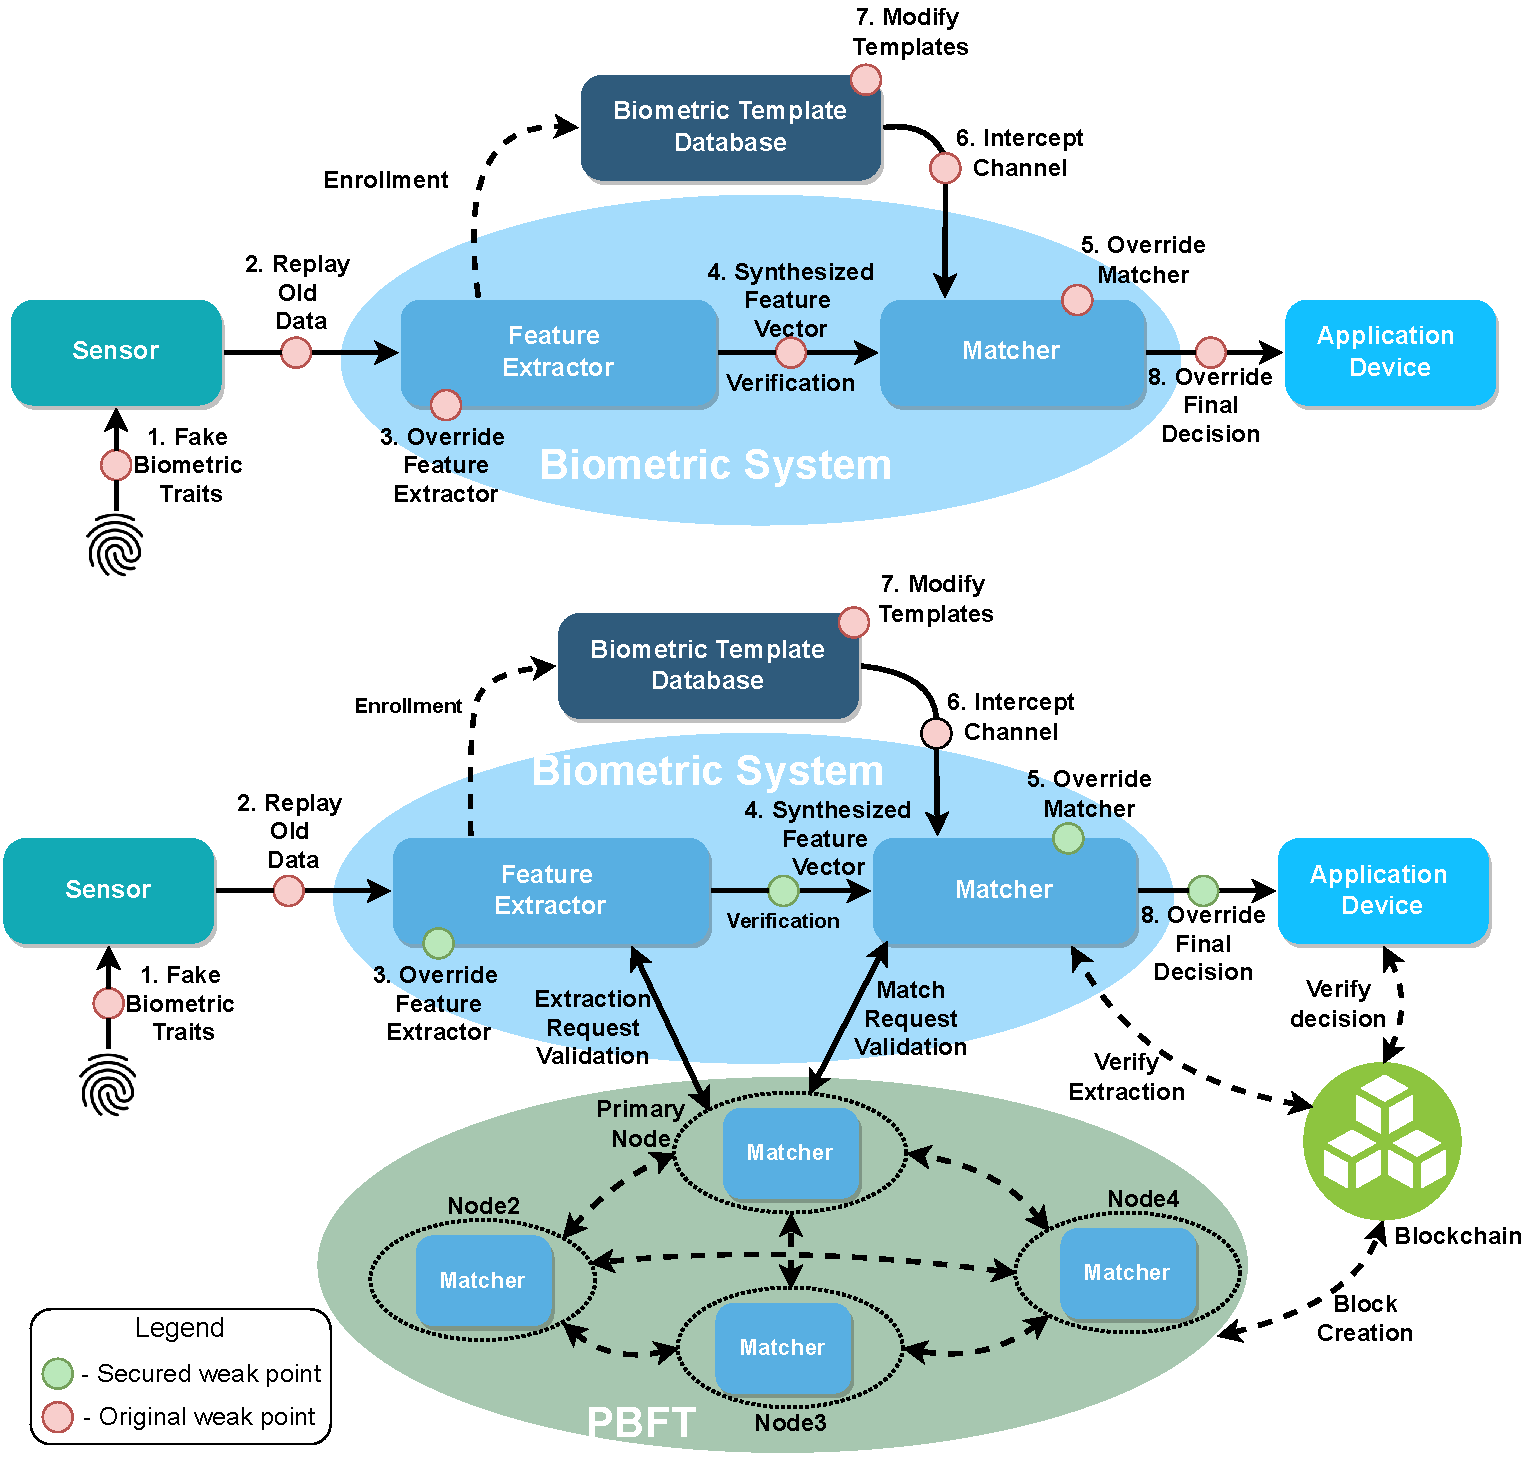
\includegraphics[width=\linewidth]{obrazky-figures/BiometricSystemComparisonWithOurDesign.pdf}
	\caption{Classical biometric system compared proposed system.}
	\label{ComparisonOfSystems}
\end{figure*}

\chapter{Conclusion and future work}
The goal of this thesis was to identify weaknesses in the security of biometric systems and design a decentralized variant that could make the system more secure. The proposed decentralized version of the biometric system, distributes the operation of the matching and feature extraction components among more nodes. The system assumes use within a single organizational, so utilization of a private blockchain infrastructure with the PBFT consensus protocol was selected. Each node in the network executes a component operation and reaches a consensus based on voting according to the PBFT protocol. Afterward, the result with other operational data is formed into a transaction and inserted into blocks that are validated between all nodes. When a consensus is reached, the block is stored on the blockchain. The blockchain is then used to provide a reliable source of proof that specific operations were executed. The design has ensured that no sensitive biometric data will be stored on the blockchain by only using it as secondary storage, where the identifiers of certain biometrics are stored. The PBFT protocol used for consensus was modified by adding node ``weights'', thus making it possible to customize the voting power of certain nodes according to the probability that the node may become compromised. 

Implemented proof-of-concept program of the proposed system, demonstrates and tests the security benefits with a broad range of testing scenarios that could occur in the classical biometric system, such as channel interception, matcher overriding, or node malfunction. Evaluation of the test scenarios has shown that decentralized design eliminates the ``single point of failure''. It is capable of minimizing the threat, where the attacker could override the feature extraction and matching module. Furthermore, the use of blockchain made it possible to withstand attacks on channels between the feature extractor, the matching, and the external application modules (see Figure \ref{ComparisonOfSystems}).
For future work, incorporation of load-balancing methods that would reduce the overall bandwidth and communication overhead of the PBFT consensus in the current system should be investigated. Another possible solution could be the combination of a public blockchain with a private blockchain, which would integrate the advantages of both to optimize throughput, latency, and scalability. For example, a combination of Proof of Stake and PBFT, where the number of consensus nodes is dynamically selected according to its equity and verifiable cryptographic sorting algorithm \cite{HybridPoSPBFT}. Another potential area of development is incorporation of dynamic weight adaptation of consensus nodes depending on accuracy and reliability. The weights would be evaluated and updated after reaching consensus and then stored on the blockchain, replacing the storage and manual management of the weights by the central authority.